% Options for packages loaded elsewhere
\PassOptionsToPackage{unicode}{hyperref}
\PassOptionsToPackage{hyphens}{url}
\PassOptionsToPackage{dvipsnames,svgnames,x11names}{xcolor}
\documentclass[
  12pt,
  a4paper,
]{article}
\usepackage{xcolor}
\usepackage[top=2.5cm,bottom=2.5cm,left=3cm,right=2cm]{geometry}
\usepackage{amsmath,amssymb}
\setcounter{secnumdepth}{5}
\usepackage{iftex}
\ifPDFTeX
  \usepackage[T1]{fontenc}
  \usepackage[utf8]{inputenc}
  \usepackage{textcomp} % provide euro and other symbols
\else % if luatex or xetex
  \usepackage{unicode-math} % this also loads fontspec
  \defaultfontfeatures{Scale=MatchLowercase}
  \defaultfontfeatures[\rmfamily]{Ligatures=TeX,Scale=1}
\fi
\usepackage{lmodern}
\ifPDFTeX\else
  % xetex/luatex font selection
    \setmainfont[]{Times New Roman}
    \setmonofont[Scale=0.85]{Liberation Mono}
\fi
% Use upquote if available, for straight quotes in verbatim environments
\IfFileExists{upquote.sty}{\usepackage{upquote}}{}
\IfFileExists{microtype.sty}{% use microtype if available
  \usepackage[]{microtype}
  \UseMicrotypeSet[protrusion]{basicmath} % disable protrusion for tt fonts
}{}
\makeatletter
\@ifundefined{KOMAClassName}{% if non-KOMA class
  \IfFileExists{parskip.sty}{%
    \usepackage{parskip}
  }{% else
    \setlength{\parindent}{0pt}
    \setlength{\parskip}{6pt plus 2pt minus 1pt}}
}{% if KOMA class
  \KOMAoptions{parskip=half}}
\makeatother
\usepackage{color}
\usepackage{fancyvrb}
\newcommand{\VerbBar}{|}
\newcommand{\VERB}{\Verb[commandchars=\\\{\}]}
\DefineVerbatimEnvironment{Highlighting}{Verbatim}{commandchars=\\\{\}}
% Add ',fontsize=\small' for more characters per line
\newenvironment{Shaded}{}{}
\newcommand{\AlertTok}[1]{\textcolor[rgb]{1.00,0.00,0.00}{\textbf{#1}}}
\newcommand{\AnnotationTok}[1]{\textcolor[rgb]{0.38,0.63,0.69}{\textbf{\textit{#1}}}}
\newcommand{\AttributeTok}[1]{\textcolor[rgb]{0.49,0.56,0.16}{#1}}
\newcommand{\BaseNTok}[1]{\textcolor[rgb]{0.25,0.63,0.44}{#1}}
\newcommand{\BuiltInTok}[1]{\textcolor[rgb]{0.00,0.50,0.00}{#1}}
\newcommand{\CharTok}[1]{\textcolor[rgb]{0.25,0.44,0.63}{#1}}
\newcommand{\CommentTok}[1]{\textcolor[rgb]{0.38,0.63,0.69}{\textit{#1}}}
\newcommand{\CommentVarTok}[1]{\textcolor[rgb]{0.38,0.63,0.69}{\textbf{\textit{#1}}}}
\newcommand{\ConstantTok}[1]{\textcolor[rgb]{0.53,0.00,0.00}{#1}}
\newcommand{\ControlFlowTok}[1]{\textcolor[rgb]{0.00,0.44,0.13}{\textbf{#1}}}
\newcommand{\DataTypeTok}[1]{\textcolor[rgb]{0.56,0.13,0.00}{#1}}
\newcommand{\DecValTok}[1]{\textcolor[rgb]{0.25,0.63,0.44}{#1}}
\newcommand{\DocumentationTok}[1]{\textcolor[rgb]{0.73,0.13,0.13}{\textit{#1}}}
\newcommand{\ErrorTok}[1]{\textcolor[rgb]{1.00,0.00,0.00}{\textbf{#1}}}
\newcommand{\ExtensionTok}[1]{#1}
\newcommand{\FloatTok}[1]{\textcolor[rgb]{0.25,0.63,0.44}{#1}}
\newcommand{\FunctionTok}[1]{\textcolor[rgb]{0.02,0.16,0.49}{#1}}
\newcommand{\ImportTok}[1]{\textcolor[rgb]{0.00,0.50,0.00}{\textbf{#1}}}
\newcommand{\InformationTok}[1]{\textcolor[rgb]{0.38,0.63,0.69}{\textbf{\textit{#1}}}}
\newcommand{\KeywordTok}[1]{\textcolor[rgb]{0.00,0.44,0.13}{\textbf{#1}}}
\newcommand{\NormalTok}[1]{#1}
\newcommand{\OperatorTok}[1]{\textcolor[rgb]{0.40,0.40,0.40}{#1}}
\newcommand{\OtherTok}[1]{\textcolor[rgb]{0.00,0.44,0.13}{#1}}
\newcommand{\PreprocessorTok}[1]{\textcolor[rgb]{0.74,0.48,0.00}{#1}}
\newcommand{\RegionMarkerTok}[1]{#1}
\newcommand{\SpecialCharTok}[1]{\textcolor[rgb]{0.25,0.44,0.63}{#1}}
\newcommand{\SpecialStringTok}[1]{\textcolor[rgb]{0.73,0.40,0.53}{#1}}
\newcommand{\StringTok}[1]{\textcolor[rgb]{0.25,0.44,0.63}{#1}}
\newcommand{\VariableTok}[1]{\textcolor[rgb]{0.10,0.09,0.49}{#1}}
\newcommand{\VerbatimStringTok}[1]{\textcolor[rgb]{0.25,0.44,0.63}{#1}}
\newcommand{\WarningTok}[1]{\textcolor[rgb]{0.38,0.63,0.69}{\textbf{\textit{#1}}}}
\usepackage{longtable,booktabs,array}
\usepackage{calc} % for calculating minipage widths
% Correct order of tables after \paragraph or \subparagraph
\usepackage{etoolbox}
\makeatletter
\patchcmd\longtable{\par}{\if@noskipsec\mbox{}\fi\par}{}{}
\makeatother
% Allow footnotes in longtable head/foot
\IfFileExists{footnotehyper.sty}{\usepackage{footnotehyper}}{\usepackage{footnote}}
\makesavenoteenv{longtable}
\usepackage{graphicx}
\makeatletter
\newsavebox\pandoc@box
\newcommand*\pandocbounded[1]{% scales image to fit in text height/width
  \sbox\pandoc@box{#1}%
  \Gscale@div\@tempa{\textheight}{\dimexpr\ht\pandoc@box+\dp\pandoc@box\relax}%
  \Gscale@div\@tempb{\linewidth}{\wd\pandoc@box}%
  \ifdim\@tempb\p@<\@tempa\p@\let\@tempa\@tempb\fi% select the smaller of both
  \ifdim\@tempa\p@<\p@\scalebox{\@tempa}{\usebox\pandoc@box}%
  \else\usebox{\pandoc@box}%
  \fi%
}
% Set default figure placement to htbp
\def\fps@figure{htbp}
\makeatother
\ifLuaTeX
\usepackage[bidi=basic]{babel}
\else
\usepackage[bidi=default]{babel}
\fi
\babelprovide[main,import]{vietnamese}
\ifPDFTeX
\else
\babelfont{rm}[]{Times New Roman}
\fi
% get rid of language-specific shorthands (see #6817):
\let\LanguageShortHands\languageshorthands
\def\languageshorthands#1{}
\setlength{\emergencystretch}{3em} % prevent overfull lines
\providecommand{\tightlist}{%
  \setlength{\itemsep}{0pt}\setlength{\parskip}{0pt}}
\usepackage{fvextra}
\DefineVerbatimEnvironment{Highlighting}{Verbatim}{breaklines,breakanywhere,commandchars=\\\{\}}
\fvset{breaklines,breakanywhere}
\usepackage{float}
\floatplacement{figure}{H}
\usepackage[font=small,labelfont=bf,labelsep=period]{caption}
\usepackage{setspace}
\setstretch{1.2}
\usepackage{fancyhdr}
\pagestyle{fancy}
\fancyhf{}
\fancyhead[L]{\small\nouppercase{\leftmark}}
\fancyhead[R]{\small Báo cáo thực hành Data Engineering}
\fancyfoot[C]{\small\thepage}
\renewcommand{\headrulewidth}{0.4pt}
\AtBeginDocument{%
  \renewcommand{\figurename}{Hình}%
  \renewcommand{\tablename}{Bảng}%
  \renewcommand{\contentsname}{Mục lục}%
  \renewcommand{\listfigurename}{Danh mục hình}%
  \renewcommand{\listtablename}{Danh mục bảng}%
  \providecommand{\chaptername}{}\renewcommand{\chaptername}{Chương}%
}
% Symbols missing from Times New Roman: typeset them in math mode instead.
\begingroup
\catcode`⌈=\active \catcode`⌉=\active \catcode`≫=\active \catcode`≪=\active
\protected\gdef⌈{\ensuremath{\lceil}}\protected\gdef⌉{\ensuremath{\rceil}}
\protected\gdef≫{\ensuremath{\gg}}\protected\gdef≪{\ensuremath{\ll}}
\endgroup
\AtBeginDocument{\catcode`⌈=\active \catcode`⌉=\active \catcode`≫=\active \catcode`≪=\active}
\usepackage{bookmark}
\IfFileExists{xurl.sty}{\usepackage{xurl}}{} % add URL line breaks if available
\urlstyle{same}
\hypersetup{
  pdflang={vi},
  colorlinks=true,
  linkcolor={black},
  filecolor={Maroon},
  citecolor={Blue},
  urlcolor={blue},
  pdfcreator={LaTeX via pandoc}}

\author{}
\date{}

\begin{document}

\begin{titlepage}
\centering
{\large\MakeUppercase{Trường Đại học Khoa học Tự nhiên, ĐHQG-HCM}\par}
{\large\bfseries\MakeUppercase{Khoa Toán - Tin học}\par}
\vspace{0.4cm}\rule{0.55\textwidth}{0.6pt}\par
\vspace{1.2cm}
\includegraphics[width=4.5cm]{/data/logo-hcmus.png}\par
\vspace{1.2cm}
{\Large\bfseries BÁO CÁO THỰC HÀNH\par}
\vspace{0.3cm}
{\large Môn học: Kỹ thuật dữ liệu (Data Engineering)\par}
\vspace{1.5cm}
{\large\bfseries Bài thực hành L06\par}
\vspace{0.4cm}
{\LARGE\bfseries Tối ưu hiệu năng Spark: shuffle, chiến lược join, data
skew, AQE, phân vùng và cache\par}
\vfill
\begin{tabular}{@{}ll@{}}
Sinh viên thực hiện:  & Nguyễn Thị Huyền Trang \\[2pt]
Mã số sinh viên:      & 23280092 \\[2pt]
Lớp:                  & 23KDL \\
\end{tabular}
\vfill
{\large TP. Hồ Chí Minh, Tháng 10 năm 2026\par}
\end{titlepage}

{
\hypersetup{linkcolor=black}
\setcounter{tocdepth}{3}
\tableofcontents
}
\listoffigures
\listoftables
\section*{Tóm tắt}\label{tuxf3m-tux1eaft}
\addcontentsline{toc}{section}{Tóm tắt}

Bài này đo ảnh hưởng của một số tham số tinh chỉnh Apache Spark 4.1.3
trên một máy, chế độ \texttt{local{[}4{]}}. Dữ liệu gồm tập chuyến taxi
New York tháng 01/2024 (2,964,624 dòng) và một bảng fact tổng hợp 10
triệu dòng, trong đó 60 \% số dòng có cùng một khóa. Mỗi biến thể được
ép chạy hết qua \emph{noop sink}; thời gian đo bằng đồng hồ tường, kế
hoạch vật lý cuối và thống kê task lấy từ Spark REST API. Với dữ liệu
nhỏ, 200 partition shuffle chậm hơn khoảng 6.7 lần so với 8 partition,
còn \emph{Adaptive Query Execution} (AQE) tự gộp partition và về gần mức
tinh chỉnh tay. Trong phép join bị lệch, task chậm nhất lâu hơn trung vị
khoảng 14 lần; AQE skew join rút thời gian từ 4.10 s xuống 2.22 s, trong
khi salting chỉ cắt được task chậm nhất mà thời gian tổng gần như giữ
nguyên. Cache một DataFrame đắt được dùng lại ba lần giảm thời gian ba
truy vấn từ 6.40 s xuống 0.99 s. Cuối bài là một số khuyến nghị cho job
production trên cluster 20 node.

\textbf{Từ khóa:} Apache Spark, shuffle partitions, Adaptive Query
Execution, broadcast hash join, sort-merge join, data skew, salting,
repartition, coalesce, cache.

\section{Giới thiệu}\label{sec:l06-intro}

Tốc độ một job Spark phụ thuộc nhiều vào cách dữ liệu được chia cho các
task: có bao nhiêu partition sau shuffle, planner chọn kiểu join nào,
khóa có bị lệch không, ghi ra bao nhiêu file, và kết quả trung gian có
được dùng lại không. Những lựa chọn này hay được đặt theo thói quen,
hoặc khi chậm thì người ta thêm máy. Bài lab L06 yêu cầu đo thay vì
đoán.

Năm thí nghiệm được thực hiện:

\begin{enumerate}
\def\labelenumi{\arabic{enumi}.}
\tightlist
\item
  E1: ảnh hưởng của
  \texttt{spark.}\allowbreak{}\texttt{sql.}\allowbreak{}\texttt{shuffle.}\allowbreak{}\texttt{partitions}\allowbreak{}
  và cơ chế gộp partition của AQE.
\item
  E2: \emph{broadcast hash join} so với \emph{sort-merge join}, vai trò
  của \texttt{autoBroadcastJoinThreshold}\allowbreak{} và gợi ý
  \texttt{broadcast()}.
\item
  E3: data skew trong join và hai cách xử lý là salting và AQE skew
  join.
\item
  E4: \texttt{repartition} so với \texttt{coalesce} trước khi ghi (thời
  gian, số file, mức song song).
\item
  E5: khi nào \texttt{cache}/\texttt{persist} có lợi.
\end{enumerate}

Mục~\ref{sec:l06-theory} nhắc lại phần lý thuyết cần dùng,
Mục~\ref{sec:l06-method} mô tả môi trường và cách đo,
Mục~\ref{sec:l06-results} trình bày kết quả,
Mục~\ref{sec:l06-discussion} trả lời tám câu hỏi checkpoint, và
Mục~\ref{sec:l06-conclusion} đưa ra khuyến nghị.

\section{Cơ sở lý thuyết}\label{sec:l06-theory}

\subsection{Shuffle và số partition
shuffle}\label{shuffle-vuxe0-sux1ed1-partition-shuffle}

Spark chia một truy vấn thành các stage, ranh giới là các \emph{wide
dependency} (phụ thuộc rộng) như \texttt{groupBy} hay \texttt{join}, nơi
các bản ghi cùng khóa phải được đưa về cùng một partition {[}1{]}. Khi
shuffle, phía map ghi dữ liệu đã băm theo khóa ra đĩa cục bộ, phía
reduce đọc lại thành
\texttt{spark.}\allowbreak{}\texttt{sql.}\allowbreak{}\texttt{shuffle.}\allowbreak{}\texttt{partitions}\allowbreak{}
partition (mặc định 200). Mỗi partition là một task, nên con số này
quyết định cả mức song song lẫn chi phí lập lịch. Quá ít partition thì
task to, dễ spill hoặc thiếu bộ nhớ; quá nhiều thì có hàng trăm task tí
hon mà phần chi phí khởi tạo còn lớn hơn phần việc thật {[}3{]},
{[}4{]}.

\subsection{Adaptive Query Execution}\label{adaptive-query-execution}

AQE tối ưu lại kế hoạch vật lý trong lúc chạy, dựa trên thống kê thật
của các stage shuffle đã xong (\emph{map output statistics}) thay vì ước
lượng từ kích thước file {[}3{]}. Bài này dùng ba tính năng của AQE: gộp
các partition nhỏ liền kề tới khoảng
\texttt{advisoryPartitionSizeInBytes}\allowbreak{} (nút
\texttt{AQEShuffleRead\ coalesced}\allowbreak{}), đổi sang broadcast khi
một phía thật sự nhỏ, và tách partition bị lệch trong sort-merge join
(\texttt{SortMergeJoin(skew=}\allowbreak{}\texttt{true)}\allowbreak{}).
AQE được bật mặc định từ Spark 3.2.

\subsection{Chiến lược join}\label{chiux1ebfn-lux1b0ux1ee3c-join}

Spark SQL {[}2{]} chọn kiểu join theo kích thước ước lượng của hai phía.
Broadcast hash join (BHJ) gom bảng nhỏ về driver rồi gửi một bản sao tới
mọi executor, nên bảng lớn không phải shuffle. Sort-merge join (SMJ)
shuffle cả hai phía theo khóa, sort từng partition rồi trộn.
\texttt{spark.}\allowbreak{}\texttt{sql.}\allowbreak{}\texttt{autoBroadcastJoinThreshold}\allowbreak{}
(mặc định 10 MB) quyết định khi nào broadcast được chọn tự động; đặt -1
sẽ tắt việc chọn tự động, nhưng gợi ý \texttt{broadcast()} viết trong mã
vẫn có hiệu lực.

\subsection{Data skew và salting}\label{data-skew-vuxe0-salting}

Skew xảy ra khi vài khóa chiếm phần lớn số bản ghi. Shuffle băm theo
khóa nên mọi bản ghi của một \emph{hot key} (khóa nóng) dồn vào một
partition, sinh ra một \emph{straggler} (task tụt hậu) trong khi các
core khác ngồi chờ. Dấu hiệu dễ nhận nhất là thời gian task lớn nhất
vượt xa trung vị trong cùng stage. Salting gắn thêm một khóa phụ ngẫu
nhiên cho hot key và nhân bản dòng tương ứng ở bảng dimension, để hot
key được rải ra nhiều partition {[}4{]}, {[}5{]}.

\subsection{repartition, coalesce và
cache}\label{repartition-coalesce-vuxe0-cache}

\texttt{repartition(n)} luôn shuffle để chia đều dữ liệu.
\texttt{coalesce(n)} chỉ gộp các partition có sẵn qua \emph{narrow
dependency} (phụ thuộc hẹp), không shuffle, nhưng có thể kéo giảm song
song của cả stage đứng trước nó {[}4{]}. \texttt{cache}/\texttt{persist}
giữ kết quả trung gian trong bộ nhớ hoặc trên đĩa để các action sau
không phải tính lại cả lineage {[}1{]}. Nó chỉ có lợi khi chi phí tính
lại lớn hơn chi phí materialize cộng với bộ nhớ bị chiếm.

\section{Môi trường và phương pháp thực nghiệm}\label{sec:l06-method}

\subsection{Môi trường}\label{muxf4i-trux1b0ux1eddng}

Mọi thứ chạy trong một container Docker, Spark ở chế độ local với 4
core, nên không có chi phí mạng giữa các executor
(Bảng~\ref{tbl:l06-env}).

\begin{longtable}[]{@{}
  >{\raggedright\arraybackslash}p{(\linewidth - 2\tabcolsep) * \real{0.5000}}
  >{\raggedright\arraybackslash}p{(\linewidth - 2\tabcolsep) * \real{0.5000}}@{}}
\caption{\label{tbl:l06-env}Môi trường thực nghiệm.}\tabularnewline
\toprule\noalign{}
\begin{minipage}[b]{\linewidth}\raggedright
Thành phần
\end{minipage} & \begin{minipage}[b]{\linewidth}\raggedright
Giá trị
\end{minipage} \\
\midrule\noalign{}
\endfirsthead
\toprule\noalign{}
\begin{minipage}[b]{\linewidth}\raggedright
Thành phần
\end{minipage} & \begin{minipage}[b]{\linewidth}\raggedright
Giá trị
\end{minipage} \\
\midrule\noalign{}
\endhead
\bottomrule\noalign{}
\endlastfoot
Máy chủ & Laptop 12 luồng CPU, 32 GB RAM \\
Ảo hóa & Docker Desktop trên WSL2, cấp 31 GB \\
Spark & 4.1.3 (image
\texttt{spark:}\allowbreak{}\texttt{4.}\allowbreak{}\texttt{1.}\allowbreak{}\texttt{3-python3}\allowbreak{}),
PySpark \\
Chế độ chạy & \texttt{local{[}4{]}} (4 core,
\texttt{defaultParallelism}\allowbreak{} = 4), driver 2 GB \\
Thu thập số liệu & \texttt{time.time()} quanh mỗi action; Spark REST API
(\texttt{/sql},
\texttt{/}\allowbreak{}\texttt{stages/}\allowbreak{}\texttt{.}\allowbreak{}\texttt{.}\allowbreak{}\texttt{.}\allowbreak{}\texttt{/}\allowbreak{}\texttt{taskSummary}\allowbreak{}) \\
Ngày thực hiện & 2026-10-30 \\
\end{longtable}

\subsection{Dữ liệu}\label{dux1eef-liux1ec7u}

Bảng fact tổng hợp được sinh bằng \texttt{spark.range}: 60 \% số dòng có
khóa 0 (\texttt{HOT\_SHARE\ =\ 0.6}), phần còn lại rải đều trên 200,000
khóa. Đếm lại thì được 5,998,366 dòng hot và 4,001,634 dòng thường. Các
tập dữ liệu được liệt kê ở Bảng~\ref{tbl:l06-data}.

\begin{longtable}[]{@{}
  >{\raggedright\arraybackslash}p{(\linewidth - 6\tabcolsep) * \real{0.2500}}
  >{\raggedright\arraybackslash}p{(\linewidth - 6\tabcolsep) * \real{0.2500}}
  >{\raggedright\arraybackslash}p{(\linewidth - 6\tabcolsep) * \real{0.2500}}
  >{\raggedright\arraybackslash}p{(\linewidth - 6\tabcolsep) * \real{0.2500}}@{}}
\caption{\label{tbl:l06-data}Dữ liệu thực nghiệm.}\tabularnewline
\toprule\noalign{}
\begin{minipage}[b]{\linewidth}\raggedright
Tập dữ liệu
\end{minipage} & \begin{minipage}[b]{\linewidth}\raggedright
Nguồn
\end{minipage} & \begin{minipage}[b]{\linewidth}\raggedright
Kích thước
\end{minipage} & \begin{minipage}[b]{\linewidth}\raggedright
Dùng trong
\end{minipage} \\
\midrule\noalign{}
\endfirsthead
\toprule\noalign{}
\begin{minipage}[b]{\linewidth}\raggedright
Tập dữ liệu
\end{minipage} & \begin{minipage}[b]{\linewidth}\raggedright
Nguồn
\end{minipage} & \begin{minipage}[b]{\linewidth}\raggedright
Kích thước
\end{minipage} & \begin{minipage}[b]{\linewidth}\raggedright
Dùng trong
\end{minipage} \\
\midrule\noalign{}
\endhead
\bottomrule\noalign{}
\endlastfoot
Trips &
\texttt{yellow\_}\allowbreak{}\texttt{tripdata\_}\allowbreak{}\texttt{2024-01.}\allowbreak{}\texttt{parquet}\allowbreak{}
& 2,964,624 dòng, 47.6 MiB, 3 row group & E1, E2, E4, E5 \\
Zones &
\texttt{taxi\_}\allowbreak{}\texttt{zone\_}\allowbreak{}\texttt{lookup.}\allowbreak{}\texttt{csv}\allowbreak{}
& 265 dòng & E2 \\
Fact tổng hợp &
\texttt{spark.}\allowbreak{}\texttt{range(10,}\allowbreak{}\texttt{000,}\allowbreak{}\texttt{000)}\allowbreak{},
60 \% key = 0 & 10,000,000 dòng & E3 \\
Dim tổng hợp &
\texttt{spark.}\allowbreak{}\texttt{range(200,}\allowbreak{}\texttt{000)}\allowbreak{},
cột \texttt{segment} = \texttt{seg\_\{key\ \%\ 50\}} & 200,000 dòng &
E3 \\
\end{longtable}

\subsection{Quy trình}\label{quy-truxecnh}

Script
\texttt{l06\_}\allowbreak{}\texttt{experiments.}\allowbreak{}\texttt{py}\allowbreak{}
(trích đoạn ở Phụ lục B) chạy từng biến thể theo các bước sau:

\begin{enumerate}
\def\labelenumi{\arabic{enumi}.}
\tightlist
\item
  Tạo SparkSession và chạy một \texttt{count()} để khởi động JVM, liệt
  kê file và làm nóng OS cache; lần này không tính.
\item
  Với mỗi biến thể, đặt lại cấu hình (\texttt{reset\_conf}), đổi tham số
  cần khảo sát, rồi ép thực thi bằng
  \texttt{df.}\allowbreak{}\texttt{write.}\allowbreak{}\texttt{format("noop")}\allowbreak{}
  (tính đủ nhưng không ghi file). E4 ghi Parquet thật để đếm số file; E5
  dùng \texttt{collect()} cho ba truy vấn.
\item
  Sau mỗi action, hàm
  \texttt{last\_}\allowbreak{}\texttt{sql\_}\allowbreak{}\texttt{summary()}\allowbreak{}
  gọi REST API lấy các nút của kế hoạch cuối (sau AQE), tổng số task, và
  median/max thời gian task tại stage lệch nhất (stage có hiệu max trừ
  median lớn nhất).
\item
  Tham số thay đổi: E1
  \texttt{shuffle.}\allowbreak{}\texttt{partitions}\allowbreak{}
  \(\in \{200, 8, 1\}\) khi tắt AQE và 200 khi bật AQE; E2 ngưỡng
  broadcast 10 MB, -1, và -1 kèm \texttt{broadcast()}; E3 SMJ 16
  partition tắt AQE, sau đó salting với 64 giá trị salt, sau đó AQE skew
  join với
  \texttt{advisoryPartitionSizeInBytes=}\allowbreak{}\texttt{4m}\allowbreak{},
  \texttt{skewedPartitionThresholdInBytes=}\allowbreak{}\texttt{16m}\allowbreak{},
  \texttt{skewedPartitionFactor=}\allowbreak{}\texttt{3}\allowbreak{} và
  tắt coalesce; E4 bốn cách phân vùng trước khi ghi; E5 ba phép tổng hợp
  có và không có
  \texttt{persist(MEMORY\_}\allowbreak{}\texttt{AND\_}\allowbreak{}\texttt{DISK)}\allowbreak{}.
\item
  Chúng tôi chạy cả script hai lần, kết quả nối vào \texttt{results.csv}
  (34 dòng = 2 lần × 17 biến thể). Báo cáo dùng lần chạy thứ hai; lần
  đầu để xem số liệu có ổn định không. Ở lần có cờ \texttt{-\/-hold},
  Spark UI được giữ lại để chụp kế hoạch và Summary Metrics.
\end{enumerate}

\section{Kết quả thực nghiệm}\label{sec:l06-results}

\subsection{Tổng quan hai lần
chạy}\label{tux1ed5ng-quan-hai-lux1ea7n-chux1ea1y}

Hình~\ref{fig:l06-console} là đầu ra console của lần chạy thứ hai,
Hình~\ref{fig:l06-table} là bảng Markdown script in ra ở cuối. Toàn bộ
17 biến thể được gom lại ở Bảng~\ref{tbl:l06-full}; hai cột median/max
là thời gian task ở stage lệch nhất của truy vấn. Tab SQL của phiên có
giữ UI liệt kê 31 truy vấn đã xong (Hình~\ref{fig:l06-sqllist}), và
chúng tôi dùng danh sách này để tìm kế hoạch của từng biến thể.

\begin{figure}
\centering
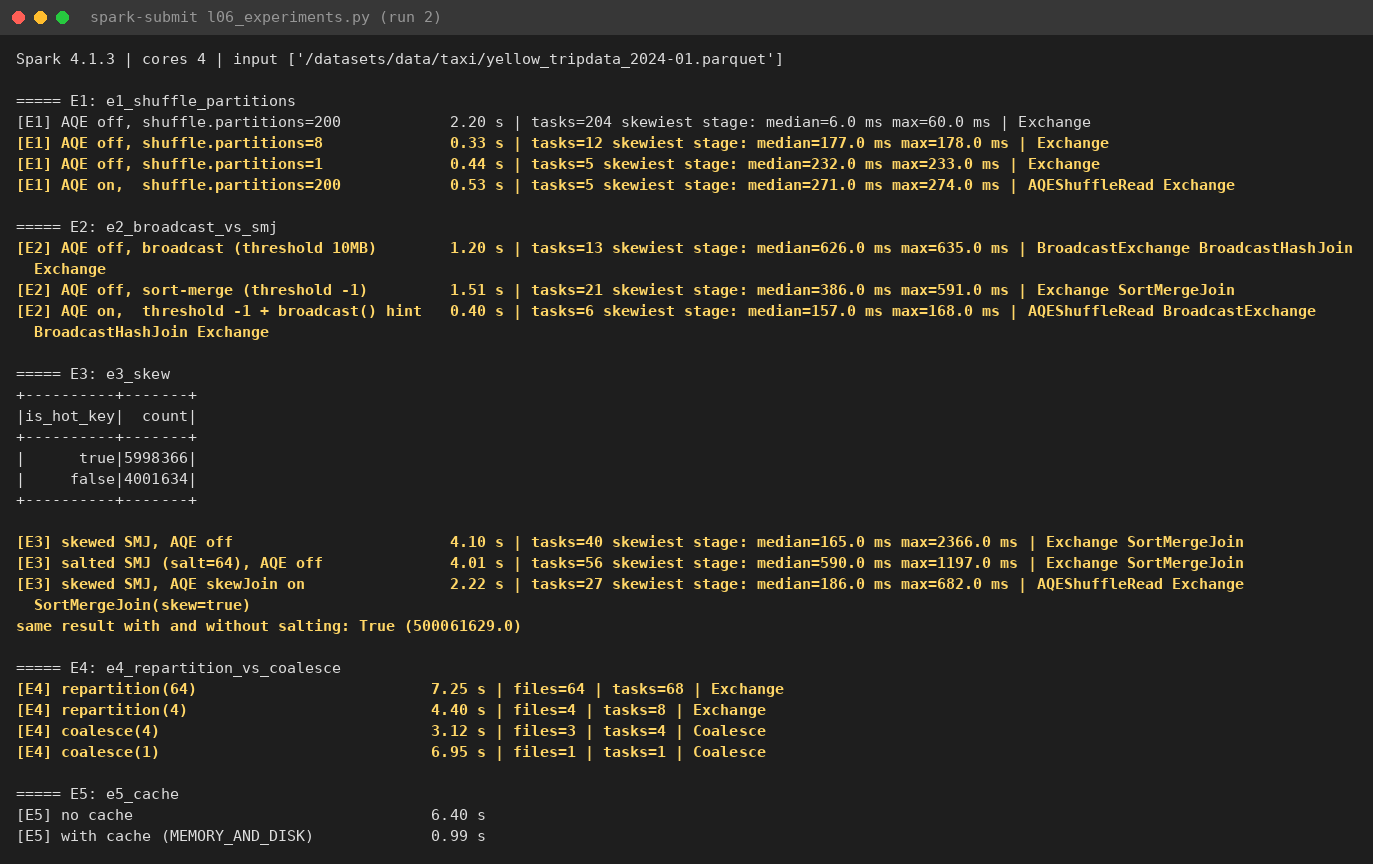
\includegraphics[width=1\linewidth,height=\textheight,keepaspectratio]{img/01_run2_console.png}
\caption{Đầu ra console của lần chạy thứ hai: thời gian, số task,
median/max task và các nút kế hoạch của từng biến
thể.}\label{fig:l06-console}
\end{figure}

\begin{figure}
\centering
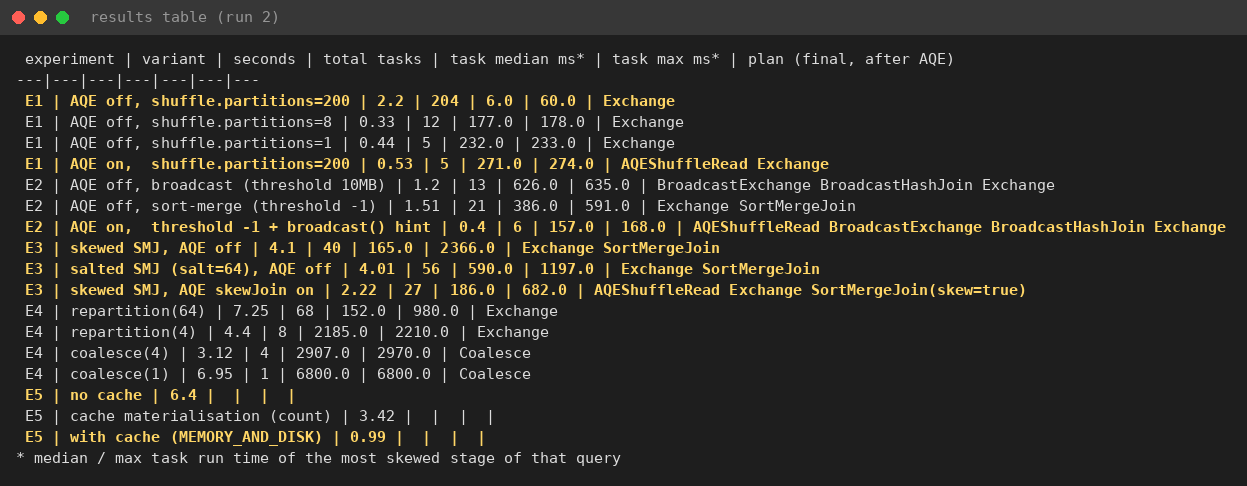
\includegraphics[width=1\linewidth,height=\textheight,keepaspectratio]{img/02_run2_results_table.png}
\caption{Bảng kết quả Markdown do script in ra ở cuối lần chạy thứ
hai.}\label{fig:l06-table}
\end{figure}

\begin{longtable}[]{@{}
  >{\raggedright\arraybackslash}p{(\linewidth - 14\tabcolsep) * \real{0.1250}}
  >{\raggedright\arraybackslash}p{(\linewidth - 14\tabcolsep) * \real{0.1250}}
  >{\raggedright\arraybackslash}p{(\linewidth - 14\tabcolsep) * \real{0.1250}}
  >{\raggedright\arraybackslash}p{(\linewidth - 14\tabcolsep) * \real{0.1250}}
  >{\raggedright\arraybackslash}p{(\linewidth - 14\tabcolsep) * \real{0.1250}}
  >{\raggedright\arraybackslash}p{(\linewidth - 14\tabcolsep) * \real{0.1250}}
  >{\raggedright\arraybackslash}p{(\linewidth - 14\tabcolsep) * \real{0.1250}}
  >{\raggedright\arraybackslash}p{(\linewidth - 14\tabcolsep) * \real{0.1250}}@{}}
\caption{\label{tbl:l06-full}Kết quả đầy đủ của lần chạy thứ hai (17
biến thể).}\tabularnewline
\toprule\noalign{}
\begin{minipage}[b]{\linewidth}\raggedright
Thí nghiệm
\end{minipage} & \begin{minipage}[b]{\linewidth}\raggedright
Biến thể
\end{minipage} & \begin{minipage}[b]{\linewidth}\raggedright
Thời gian (s)
\end{minipage} & \begin{minipage}[b]{\linewidth}\raggedright
Tổng task
\end{minipage} & \begin{minipage}[b]{\linewidth}\raggedright
Median (ms)
\end{minipage} & \begin{minipage}[b]{\linewidth}\raggedright
Max (ms)
\end{minipage} & \begin{minipage}[b]{\linewidth}\raggedright
Kế hoạch cuối
\end{minipage} & \begin{minipage}[b]{\linewidth}\raggedright
Ghi chú
\end{minipage} \\
\midrule\noalign{}
\endfirsthead
\toprule\noalign{}
\begin{minipage}[b]{\linewidth}\raggedright
Thí nghiệm
\end{minipage} & \begin{minipage}[b]{\linewidth}\raggedright
Biến thể
\end{minipage} & \begin{minipage}[b]{\linewidth}\raggedright
Thời gian (s)
\end{minipage} & \begin{minipage}[b]{\linewidth}\raggedright
Tổng task
\end{minipage} & \begin{minipage}[b]{\linewidth}\raggedright
Median (ms)
\end{minipage} & \begin{minipage}[b]{\linewidth}\raggedright
Max (ms)
\end{minipage} & \begin{minipage}[b]{\linewidth}\raggedright
Kế hoạch cuối
\end{minipage} & \begin{minipage}[b]{\linewidth}\raggedright
Ghi chú
\end{minipage} \\
\midrule\noalign{}
\endhead
\bottomrule\noalign{}
\endlastfoot
E1 & AQE off, shuffle.partitions=200 & 2.20 & 204 & 6 & 60 & Exchange
& \\
E1 & AQE off, shuffle.partitions=8 & 0.33 & 12 & 177 & 178 & Exchange
& \\
E1 & AQE off, shuffle.partitions=1 & 0.44 & 5 & 232 & 233 & Exchange
& \\
E1 & AQE on, shuffle.partitions=200 & 0.53 & 5 & 271 & 274 &
AQEShuffleRead Exchange & AQE gộp partition nhỏ \\
E2 & AQE off, broadcast (threshold 10MB) & 1.20 & 13 & 626 & 635 &
BroadcastExchange BroadcastHashJoin Exchange & \\
E2 & AQE off, sort-merge (threshold -1) & 1.51 & 21 & 386 & 591 &
Exchange SortMergeJoin & \\
E2 & AQE on, threshold -1 + broadcast() hint & 0.40 & 6 & 157 & 168 &
AQEShuffleRead BroadcastExchange BroadcastHashJoin Exchange & hint thắng
threshold \\
E3 & skewed SMJ, AQE off & 4.10 & 40 & 165 & \textbf{2366} & Exchange
SortMergeJoin & \\
E3 & salted SMJ (salt=64), AQE off & 4.01 & 56 & 590 & 1197 & Exchange
SortMergeJoin & cùng kết quả (500061629) \\
E3 & skewed SMJ, AQE skewJoin on & 2.22 & 27 & 186 & 682 &
AQEShuffleRead Exchange SortMergeJoin(skew=true) & 1 partition skew, 4
split \\
E4 & repartition(64) & 7.25 & 68 & 152 & 980 & Exchange & 64 file \\
E4 & repartition(4) & 4.40 & 8 & 2185 & 2210 & Exchange & 4 file \\
E4 & coalesce(4) & 3.12 & 4 & 2907 & 2970 & Coalesce & 3 file \\
E4 & coalesce(1) & 6.95 & 1 & 6800 & 6800 & Coalesce & 1 file \\
E5 & no cache (3 queries) & 6.40 & & & & & 3 aggregation \\
E5 & cache materialisation (count) & 3.42 & & & & & 2,869,714 dòng, 59.4
MiB \\
E5 & with cache (3 queries) & 0.99 & & & & & 3 aggregation \\
\end{longtable}

\begin{figure}
\centering
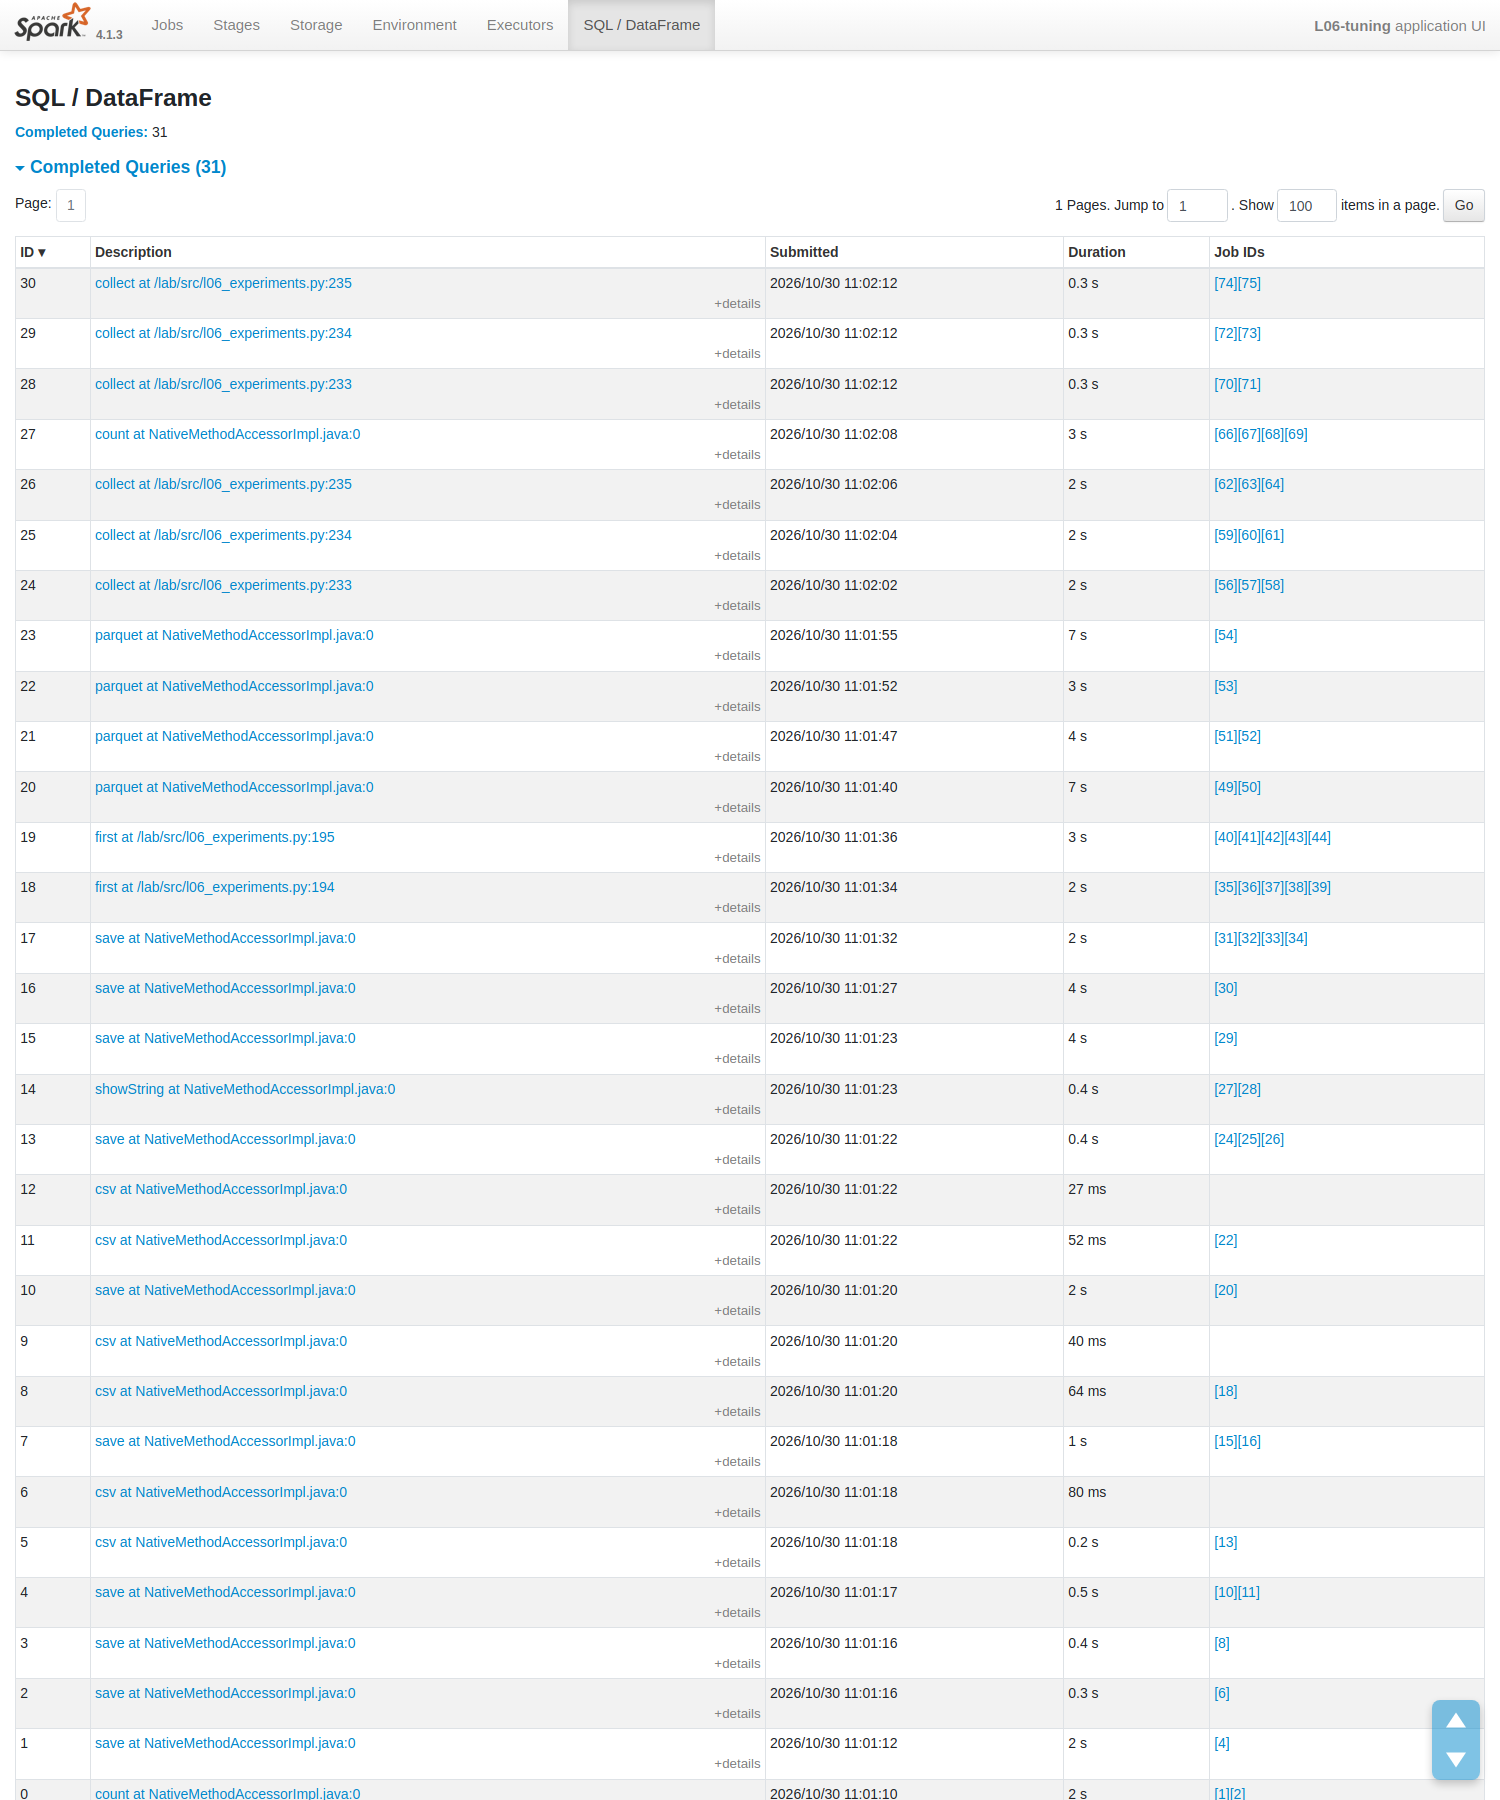
\includegraphics[width=0.85\linewidth,height=\textheight,keepaspectratio]{img/20_ui_sql_list.png}
\caption{Tab SQL / DataFrame của Spark UI với 31 truy vấn đã hoàn tất
trong phiên chạy.}\label{fig:l06-sqllist}
\end{figure}

Lần chạy đầu (tổng 71.71 s) cho cùng xu hướng ở mọi thí nghiệm
(Bảng~\ref{tbl:l06-runs}). Phần lớn chênh lệch nằm trong khoảng ±20 \%
mà đề bài cho phép. Ngoại lệ là các biến thể rất ngắn: E2 broadcast khi
tắt AQE lần đầu chỉ 0.77 s, lần hai lên 1.20 s, và E1 một partition từ
0.30 s lên 0.44 s. Với truy vấn chạy dưới một giây, vài trăm mili giây
dao động đã là tỉ lệ lớn, nên chúng tôi không rút kết luận từ chênh lệch
nhỏ giữa các biến thể loại này.

\begin{longtable}[]{@{}lll@{}}
\caption{\label{tbl:l06-runs}So sánh một số chỉ số giữa hai lần
chạy.}\tabularnewline
\toprule\noalign{}
Chỉ số & Lần 1 & Lần 2 \\
\midrule\noalign{}
\endfirsthead
\toprule\noalign{}
Chỉ số & Lần 1 & Lần 2 \\
\midrule\noalign{}
\endhead
\bottomrule\noalign{}
\endlastfoot
E1, 200 partition, AQE off & 2.15 s & 2.20 s \\
E2, broadcast, AQE off & 0.77 s & 1.20 s \\
E3 baseline, task max & 2,686 ms & 2,366 ms \\
E3 salting & 4.28 s & 4.01 s \\
E3 AQE skew join & 2.28 s & 2.22 s \\
E5 không cache & 6.07 s & 6.40 s \\
E5 với cache & 0.88 s & 0.99 s \\
\end{longtable}

\subsection{E1: số partition shuffle và AQE
coalescing}\label{e1-sux1ed1-partition-shuffle-vuxe0-aqe-coalescing}

Truy vấn
\texttt{groupBy(PULocationID,}\allowbreak{}\texttt{\ DOLocationID).}\allowbreak{}\texttt{agg(count,}\allowbreak{}\texttt{\ avg)}\allowbreak{}
đọc 47.6 MiB nhưng chỉ ghi khoảng 1167.1 KiB dữ liệu shuffle. Với 200
partition và AQE tắt, truy vấn sinh 204 task (4 map, 200 reduce), mỗi
task reduce chạy khoảng 6 ms, và đây là biến thể chậm nhất. Kế hoạch ở
Hình~\ref{fig:l06-e1off} chỉ có một \texttt{Exchange} 200 partition.

\begin{figure}
\centering
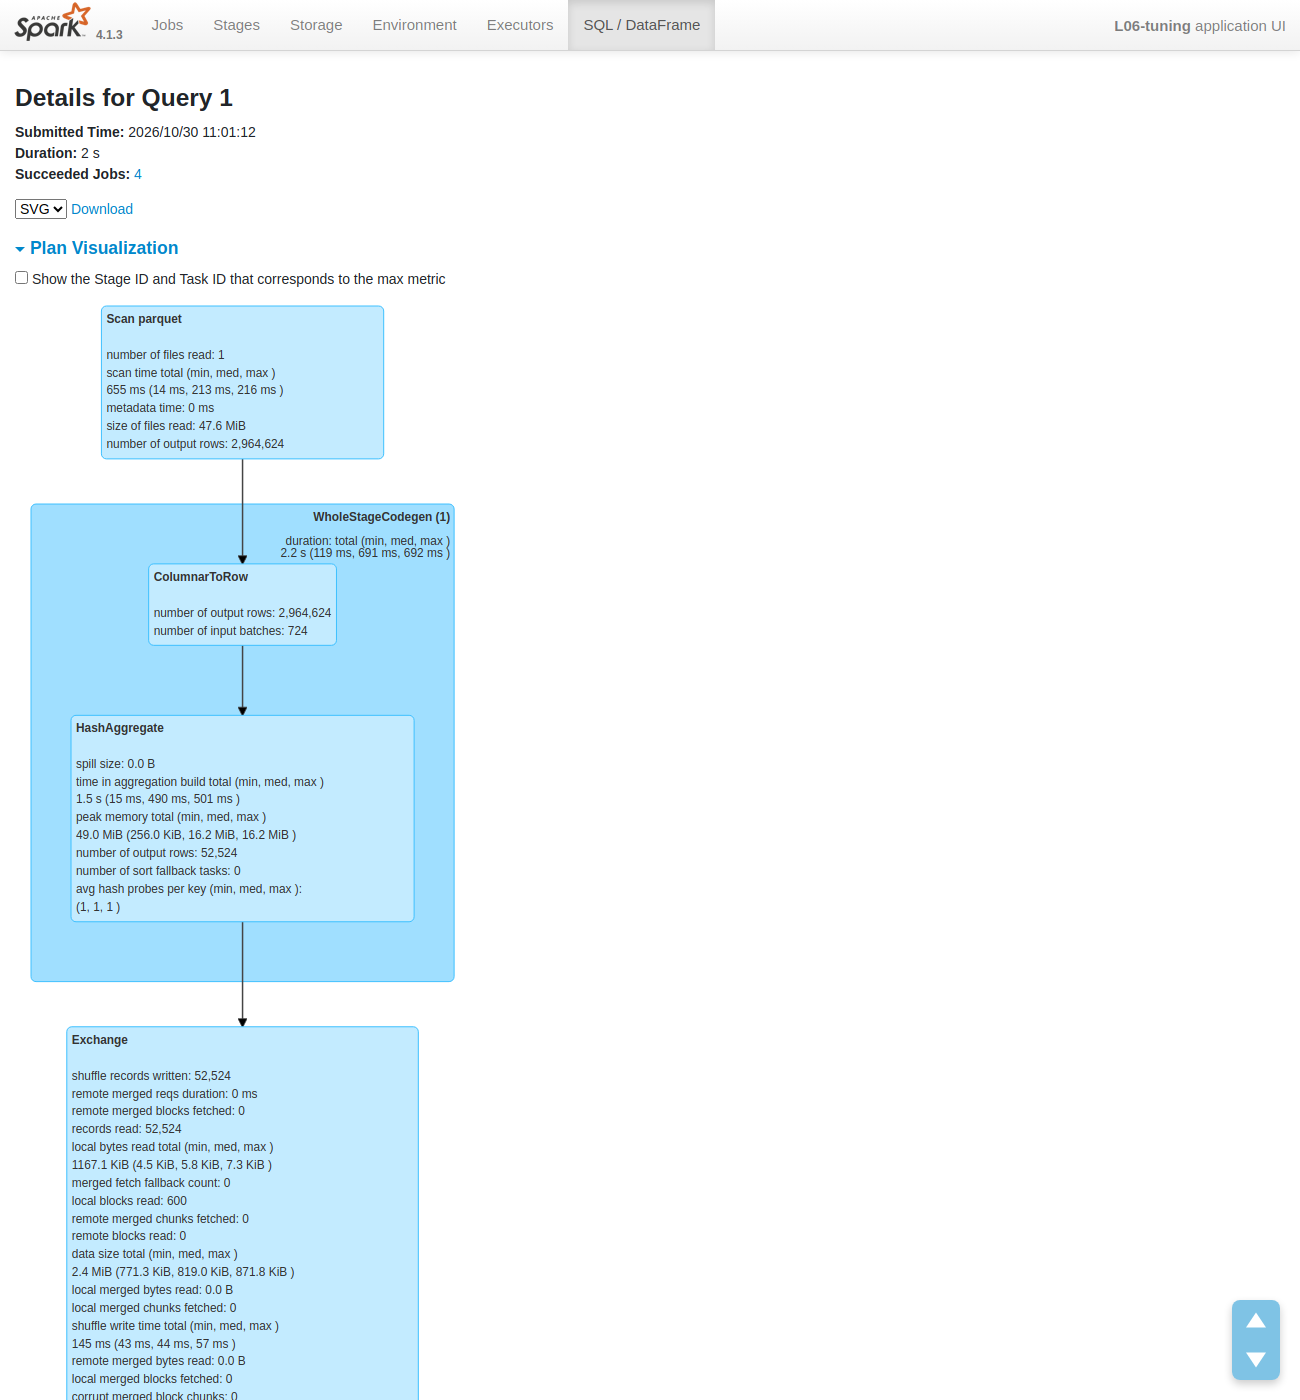
\includegraphics[width=0.7\linewidth,height=\textheight,keepaspectratio]{img/21_ui_e1_aqe_off_200.png}
\caption{Kế hoạch E1 khi AQE tắt: \texttt{Exchange} với 200 partition
shuffle.}\label{fig:l06-e1off}
\end{figure}

Bật AQE mà vẫn để 200 partition thì sau \texttt{Exchange} xuất hiện
\texttt{AQEShuffleRead} (Hình~\ref{fig:l06-e1on}), các partition nhỏ
được gộp lại, tổng chỉ còn 5 task, thời gian xấp xỉ bản tinh chỉnh tay 8
partition. Bản 1 partition cũng nhanh, nhưng chỉ vì kết quả quá nhỏ
(khoảng 20 nghìn nhóm); Mục~\ref{sec:l06-q1} giải thích vì sao không nên
dùng nó.

\begin{figure}
\centering
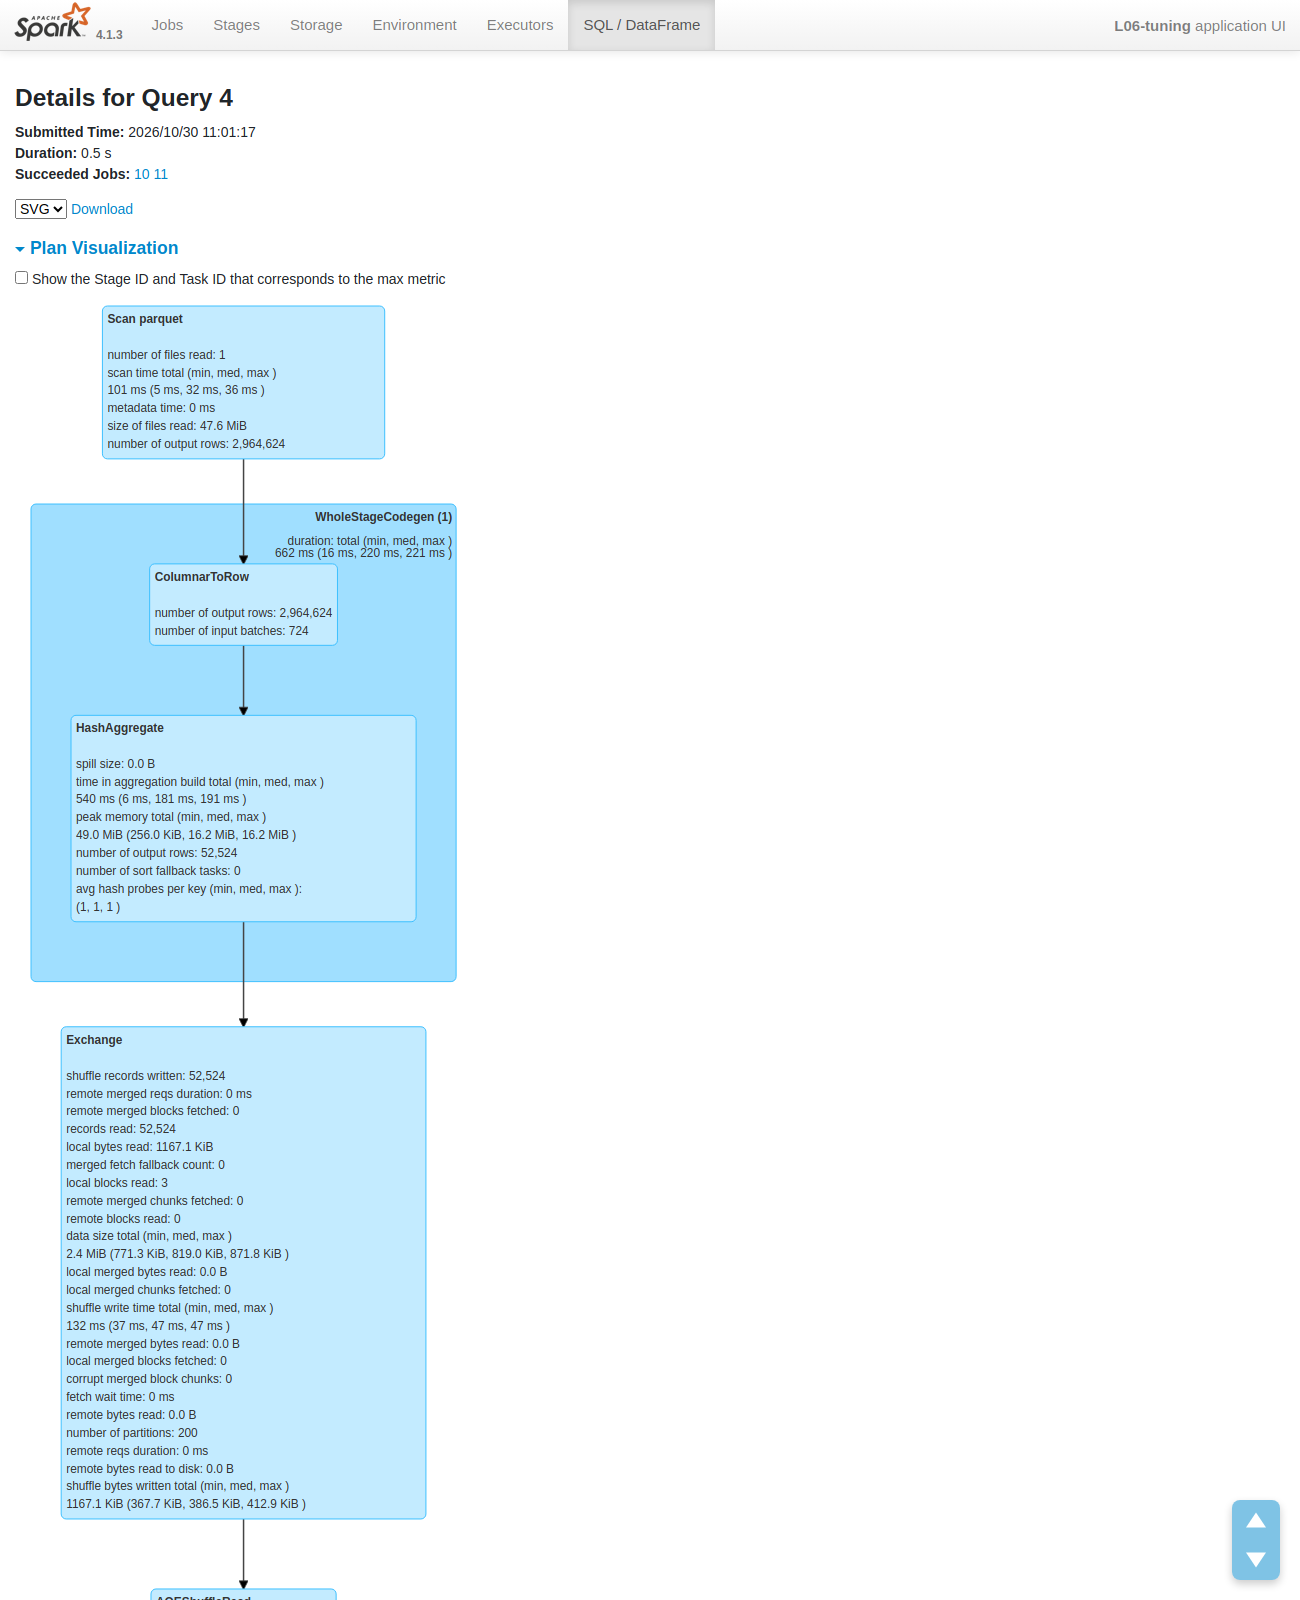
\includegraphics[width=0.7\linewidth,height=\textheight,keepaspectratio]{img/22_ui_e1_aqe_on_coalesced.png}
\caption{Kế hoạch E1 khi AQE bật: \texttt{Exchange} 200 partition theo
sau là \texttt{AQEShuffleRead} ở chế độ coalesced; truy vấn đọc
2,964,624 dòng, 47.6 MiB.}\label{fig:l06-e1on}
\end{figure}

\subsection{E2: broadcast hash join và sort-merge
join}\label{e2-broadcast-hash-join-vuxe0-sort-merge-join}

Phép join \(\text{trips} \bowtie \text{zones}\) (zones có 265 dòng) được
chạy theo ba cách. Khi ngưỡng là -1, Spark phải dùng
\texttt{SortMergeJoin}: khoảng 3 triệu chuyến bị shuffle cùng bảng zone
rồi sort (Hình~\ref{fig:l06-e2smj}). Khi broadcast, chỉ 265 dòng được
gửi đi và phía trips không có \texttt{Exchange} trước join
(Hình~\ref{fig:l06-e2bhj}).

\begin{figure}
\centering
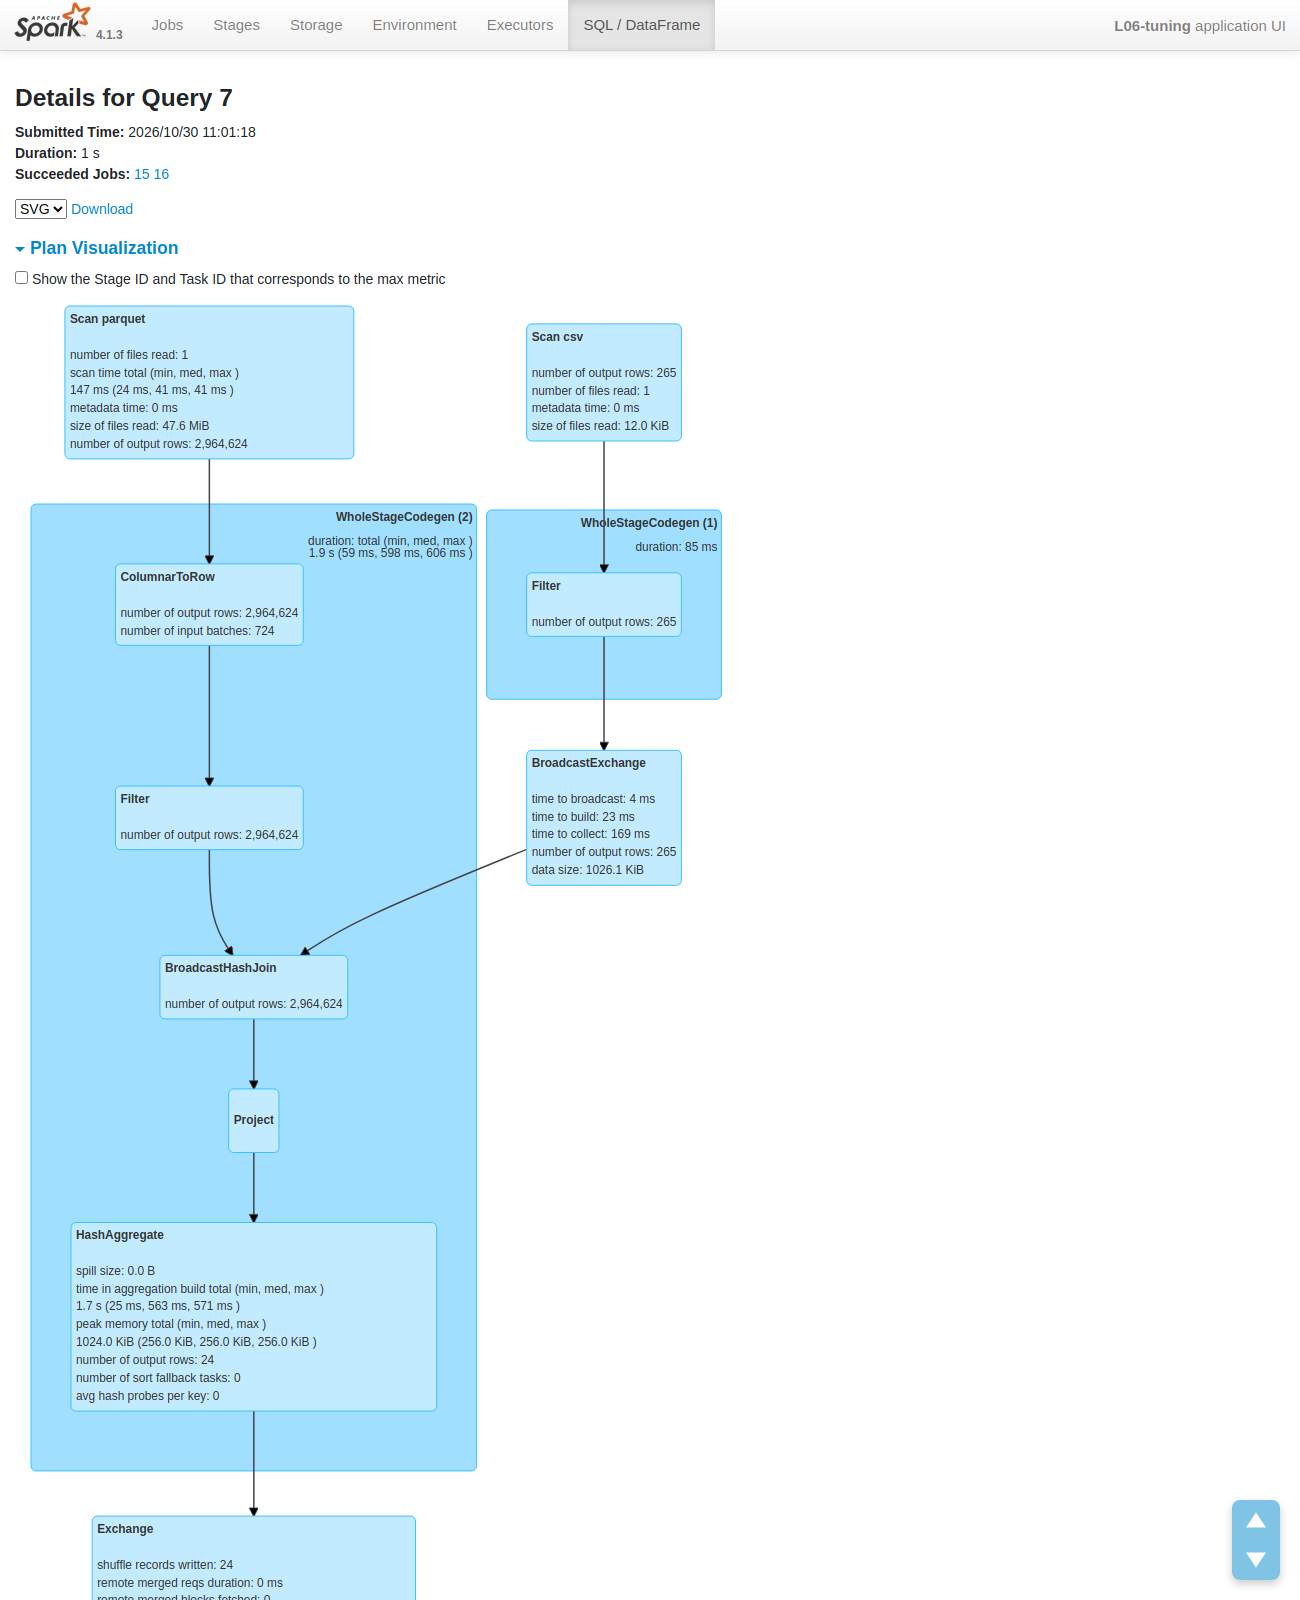
\includegraphics[width=0.85\linewidth,height=\textheight,keepaspectratio]{img/23_ui_e2_broadcast.png}
\caption{Kế hoạch E2 với broadcast:
\texttt{BroadcastExchange}\allowbreak{} và
\texttt{BroadcastHashJoin}\allowbreak{}, phía trips không có
\texttt{Exchange} trước join.}\label{fig:l06-e2bhj}
\end{figure}

\begin{figure}
\centering
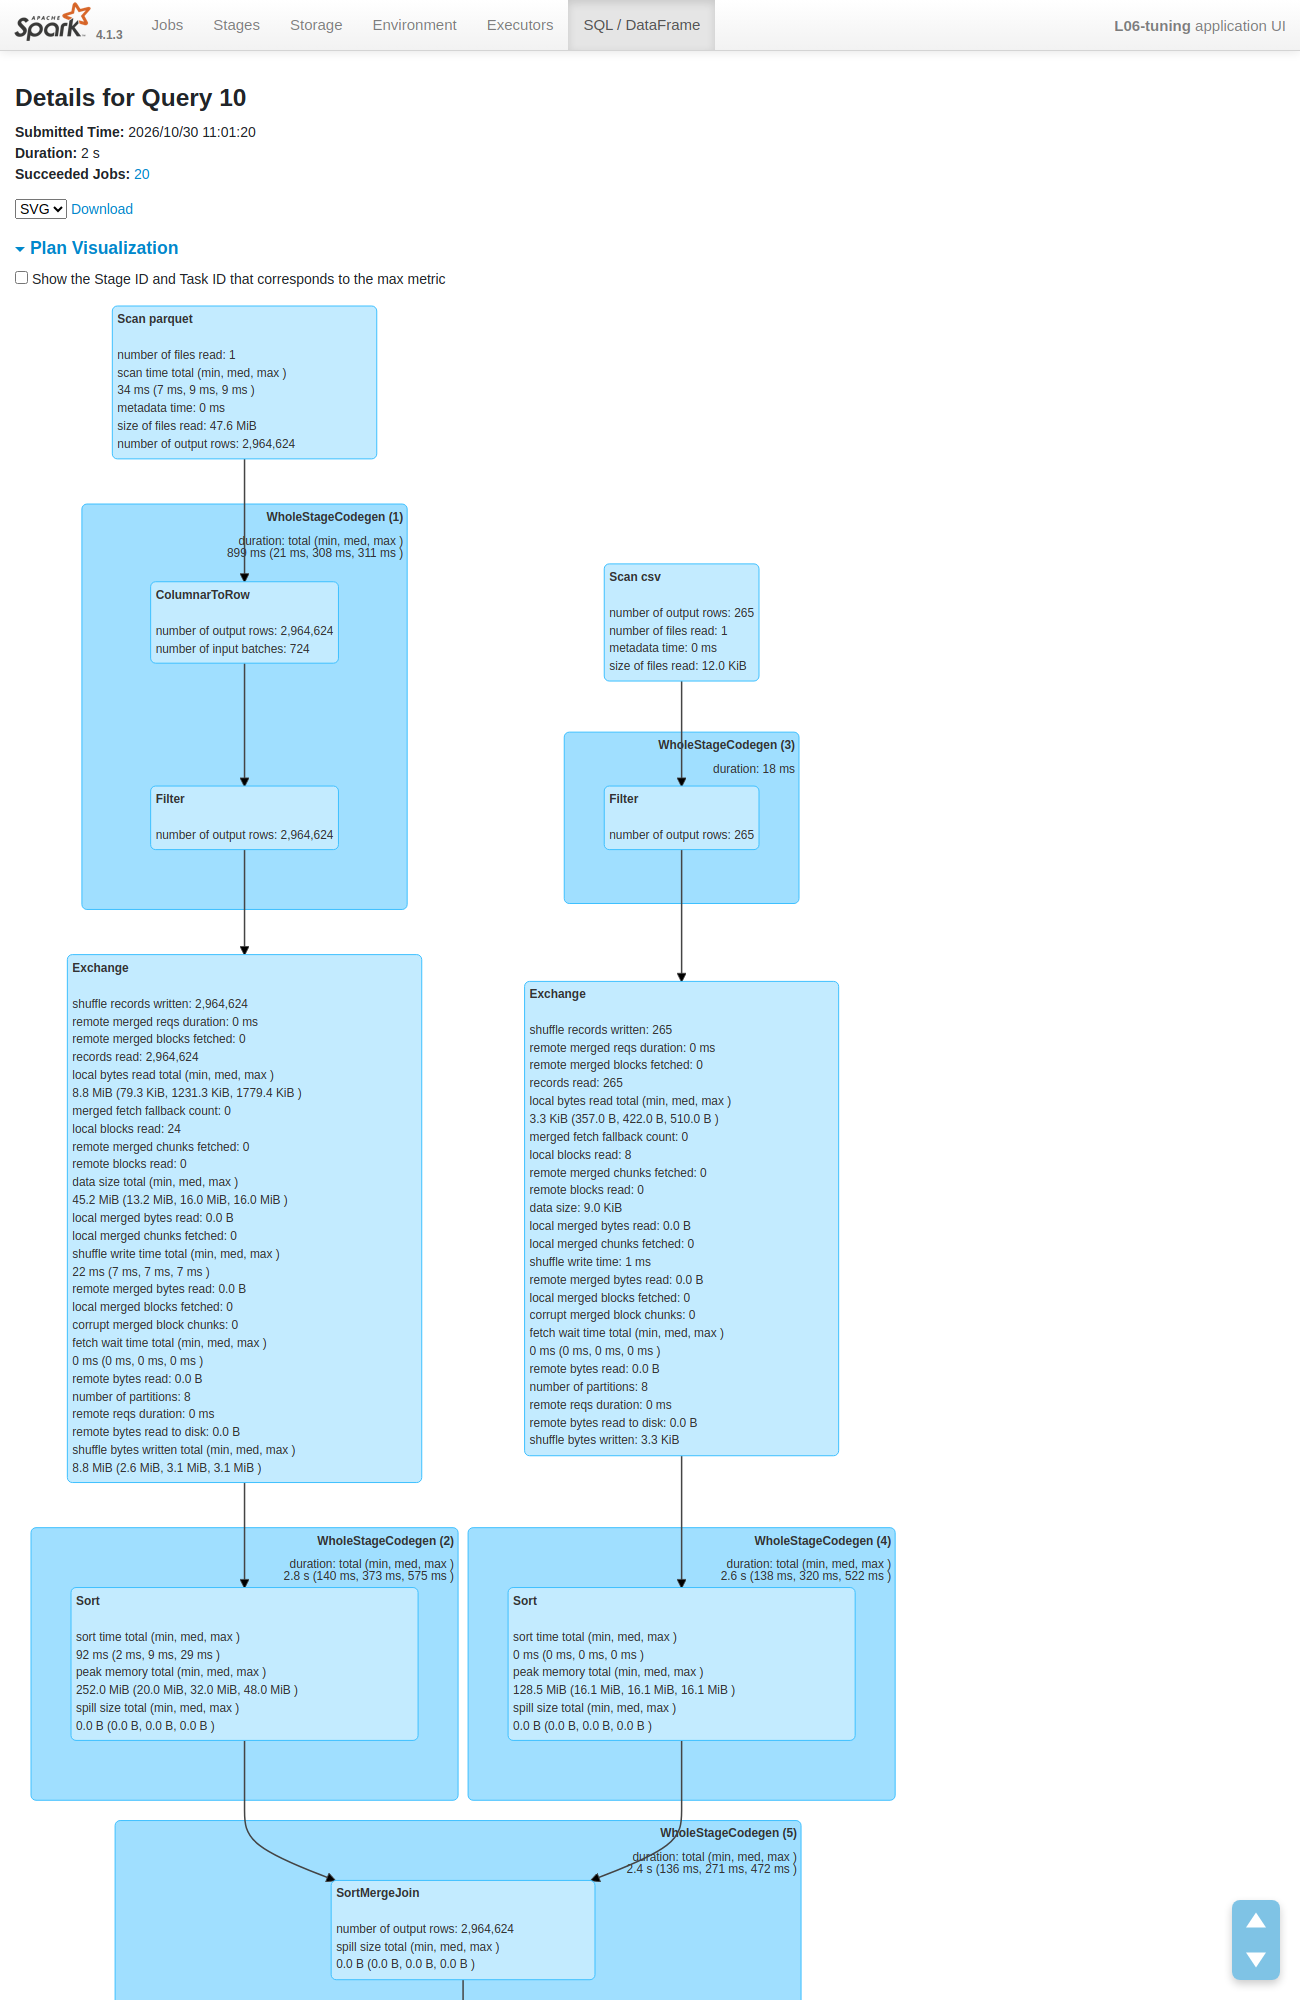
\includegraphics[width=1\linewidth,height=\textheight,keepaspectratio]{img/24_ui_e2_sortmerge.png}
\caption{Kế hoạch E2 với ngưỡng -1: \texttt{Exchange} và \texttt{Sort} ở
cả hai phía trước \texttt{SortMergeJoin}.}\label{fig:l06-e2smj}
\end{figure}

Gợi ý \texttt{F.broadcast()} vẫn có tác dụng khi ngưỡng là -1 và là biến
thể nhanh nhất của E2 (0.40 s, 6 task). Chúng tôi hơi bất ngờ khi thấy
broadcast tắt AQE (1.20 s) chỉ nhanh hơn SMJ (1.51 s) một chút. Lý do có
lẽ là cấu hình mặc định của script chỉ dùng 8 partition nên SMJ ở đây
khá nhẹ, cộng thêm dao động giữa các lần chạy đã nói ở trên. Khác biệt
thật nằm ở kế hoạch: broadcast bỏ được \texttt{Exchange} và
\texttt{Sort} ở phía bảng lớn, và khoản tiết kiệm này sẽ lớn dần theo
kích thước dữ liệu.

\subsection{E3: data skew, salting và AQE skew
join}\label{e3-data-skew-salting-vuxe0-aqe-skew-join}

Bảng fact có 5,998,366 dòng mang khóa 0. Bằng REST API, chúng tôi lấy
phân vị thời gian task và số bản ghi shuffle đọc mỗi task tại stage join
của ba biến thể (Bảng~\ref{tbl:l06-quantiles},
Hình~\ref{fig:l06-quantiles}).

\begin{longtable}[]{@{}
  >{\raggedright\arraybackslash}p{(\linewidth - 4\tabcolsep) * \real{0.3333}}
  >{\raggedright\arraybackslash}p{(\linewidth - 4\tabcolsep) * \real{0.3333}}
  >{\raggedright\arraybackslash}p{(\linewidth - 4\tabcolsep) * \real{0.3333}}@{}}
\caption{\label{tbl:l06-quantiles}Phân vị min / 25 \% / median / 75 \% /
max tại stage join của E3 (lần chạy thứ hai).}\tabularnewline
\toprule\noalign{}
\begin{minipage}[b]{\linewidth}\raggedright
Stage (biến thể)
\end{minipage} & \begin{minipage}[b]{\linewidth}\raggedright
Thời gian task (ms)
\end{minipage} & \begin{minipage}[b]{\linewidth}\raggedright
Bản ghi shuffle đọc / task
\end{minipage} \\
\midrule\noalign{}
\endfirsthead
\toprule\noalign{}
\begin{minipage}[b]{\linewidth}\raggedright
Stage (biến thể)
\end{minipage} & \begin{minipage}[b]{\linewidth}\raggedright
Thời gian task (ms)
\end{minipage} & \begin{minipage}[b]{\linewidth}\raggedright
Bản ghi shuffle đọc / task
\end{minipage} \\
\midrule\noalign{}
\endhead
\bottomrule\noalign{}
\endlastfoot
42: baseline, AQE off & 140 / 157 / 165 / 379 / 2,366 & 260,166 /
261,225 / 262,619 / 264,416 / 6,264,438 \\
46: salting 64 & 308 / 484 / 590 / 901 / 1,197 & 359,285 / 543,450 /
638,133 / 823,338 / 917,267 \\
52: AQE skew join & 129 / 144 / 186 / 199 / 682 & 260,166 / 261,225 /
262,677 / 265,121 / 1,576,365 \\
\end{longtable}

\begin{figure}
\centering
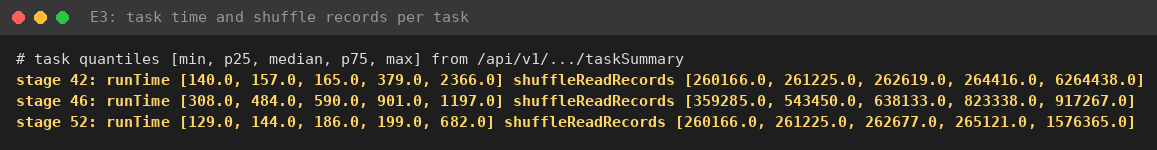
\includegraphics[width=0.85\linewidth,height=\textheight,keepaspectratio]{img/03_e3_task_quantiles.png}
\caption{Phân vị thời gian task và số bản ghi shuffle mỗi task của ba
stage join E3, lấy từ Spark REST API.}\label{fig:l06-quantiles}
\end{figure}

\emph{Baseline.} Kế hoạch là \texttt{Exchange} + \texttt{SortMergeJoin}
với 16 partition (Hình~\ref{fig:l06-e3base}). Ở stage 42, task chậm nhất
lâu hơn median khoảng 14 lần. Theo Summary Metrics
(Hình~\ref{fig:l06-stage42}), task này đọc 61.9 MiB, trong khi các task
khác chỉ khoảng 3.4 MiB. Cả stage đọc 113.0 MiB / 10,200,000 bản ghi qua
16 task. Trong lúc task đó chạy, ba core còn lại không có việc gì làm.

\begin{figure}
\centering
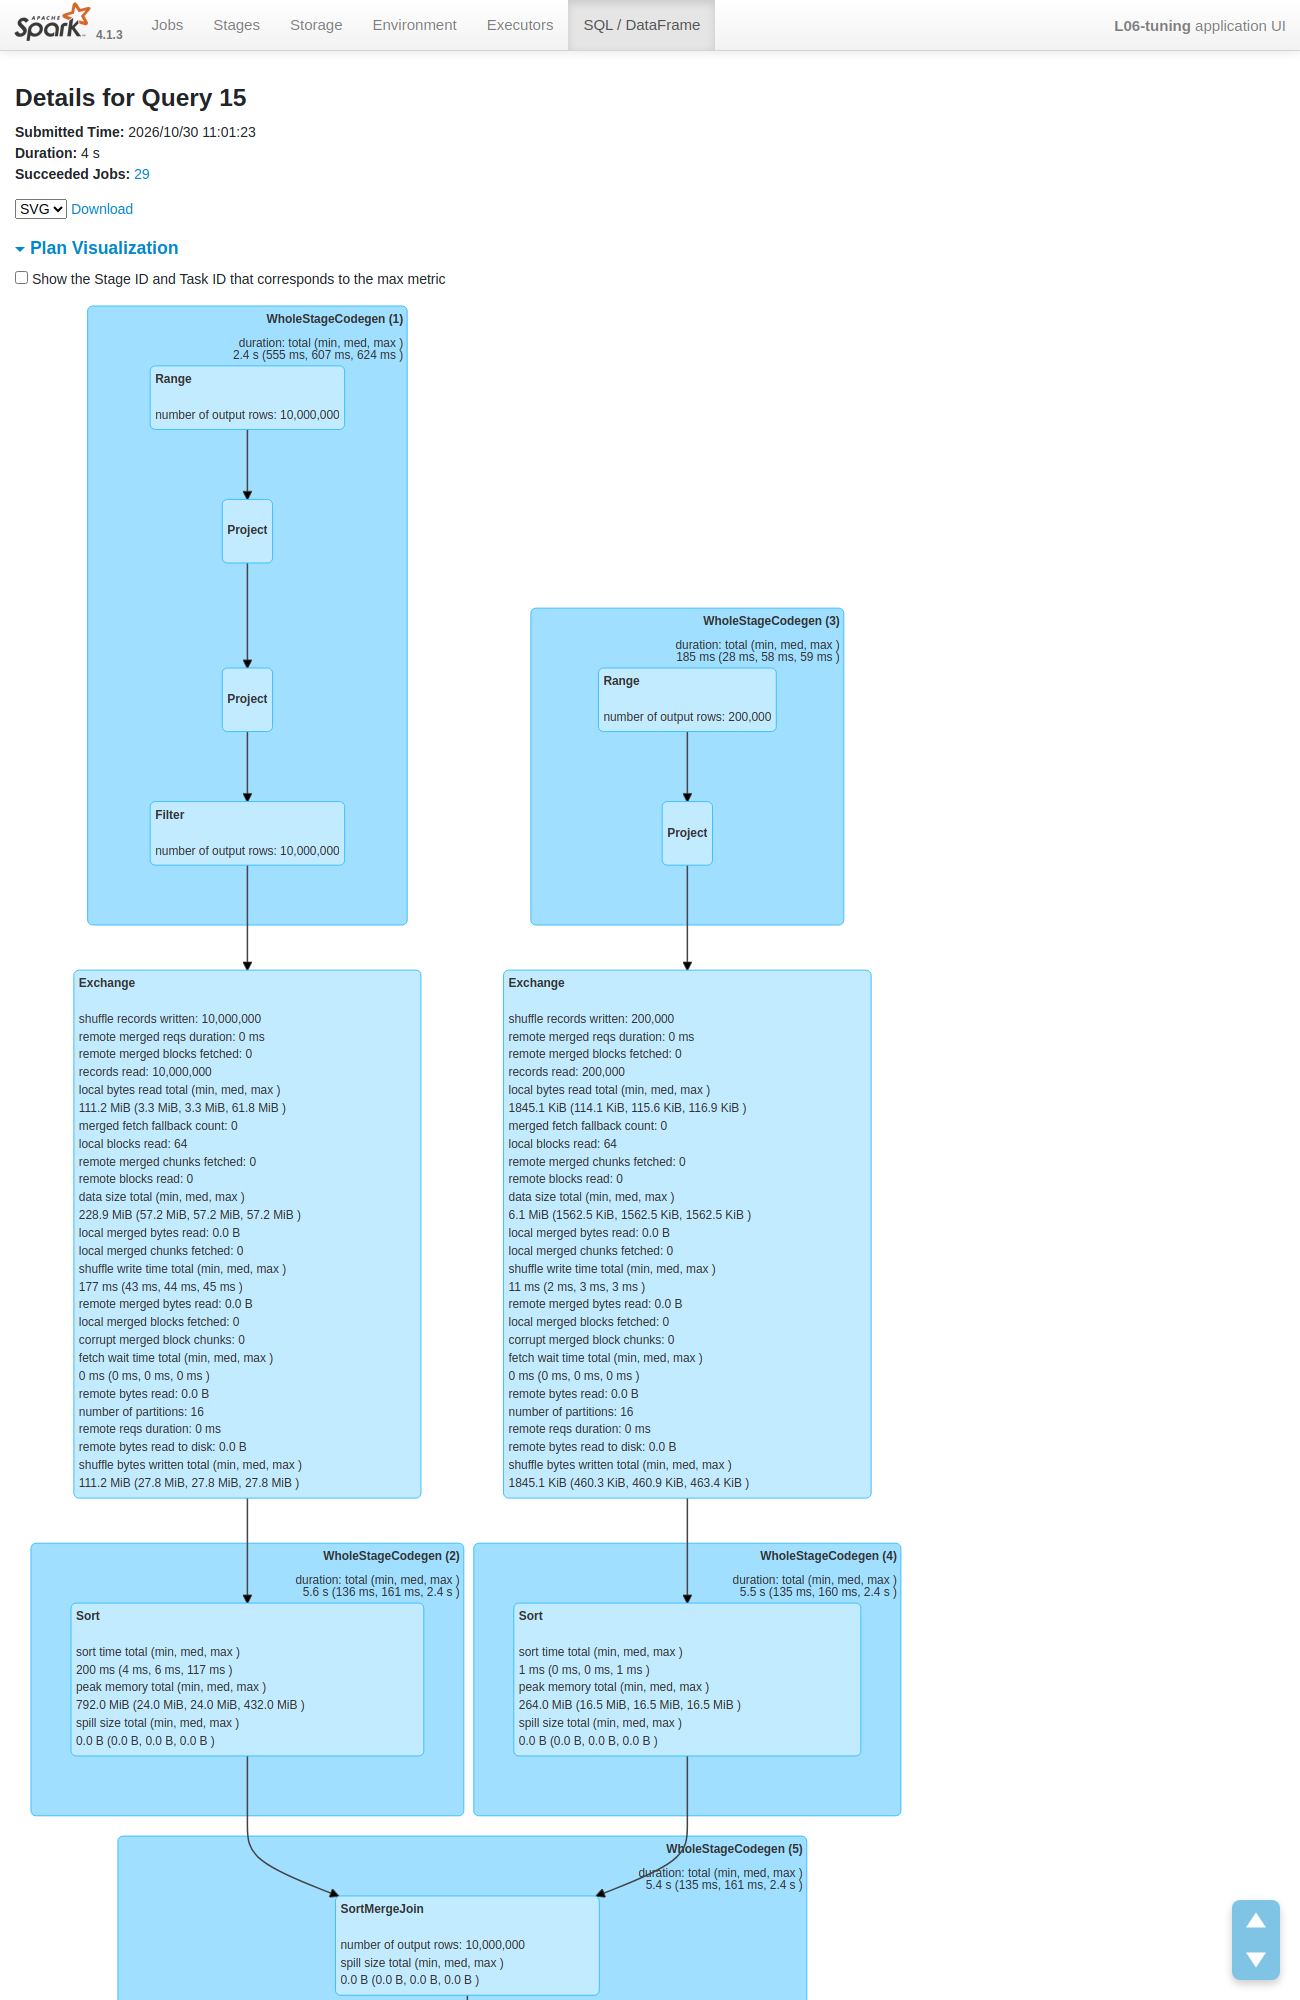
\includegraphics[width=0.85\linewidth,height=\textheight,keepaspectratio]{img/25_ui_e3_skew_baseline_smj.png}
\caption{Kế hoạch E3 baseline (AQE tắt): sort-merge join trên dữ liệu
lệch.}\label{fig:l06-e3base}
\end{figure}

\begin{figure}
\centering
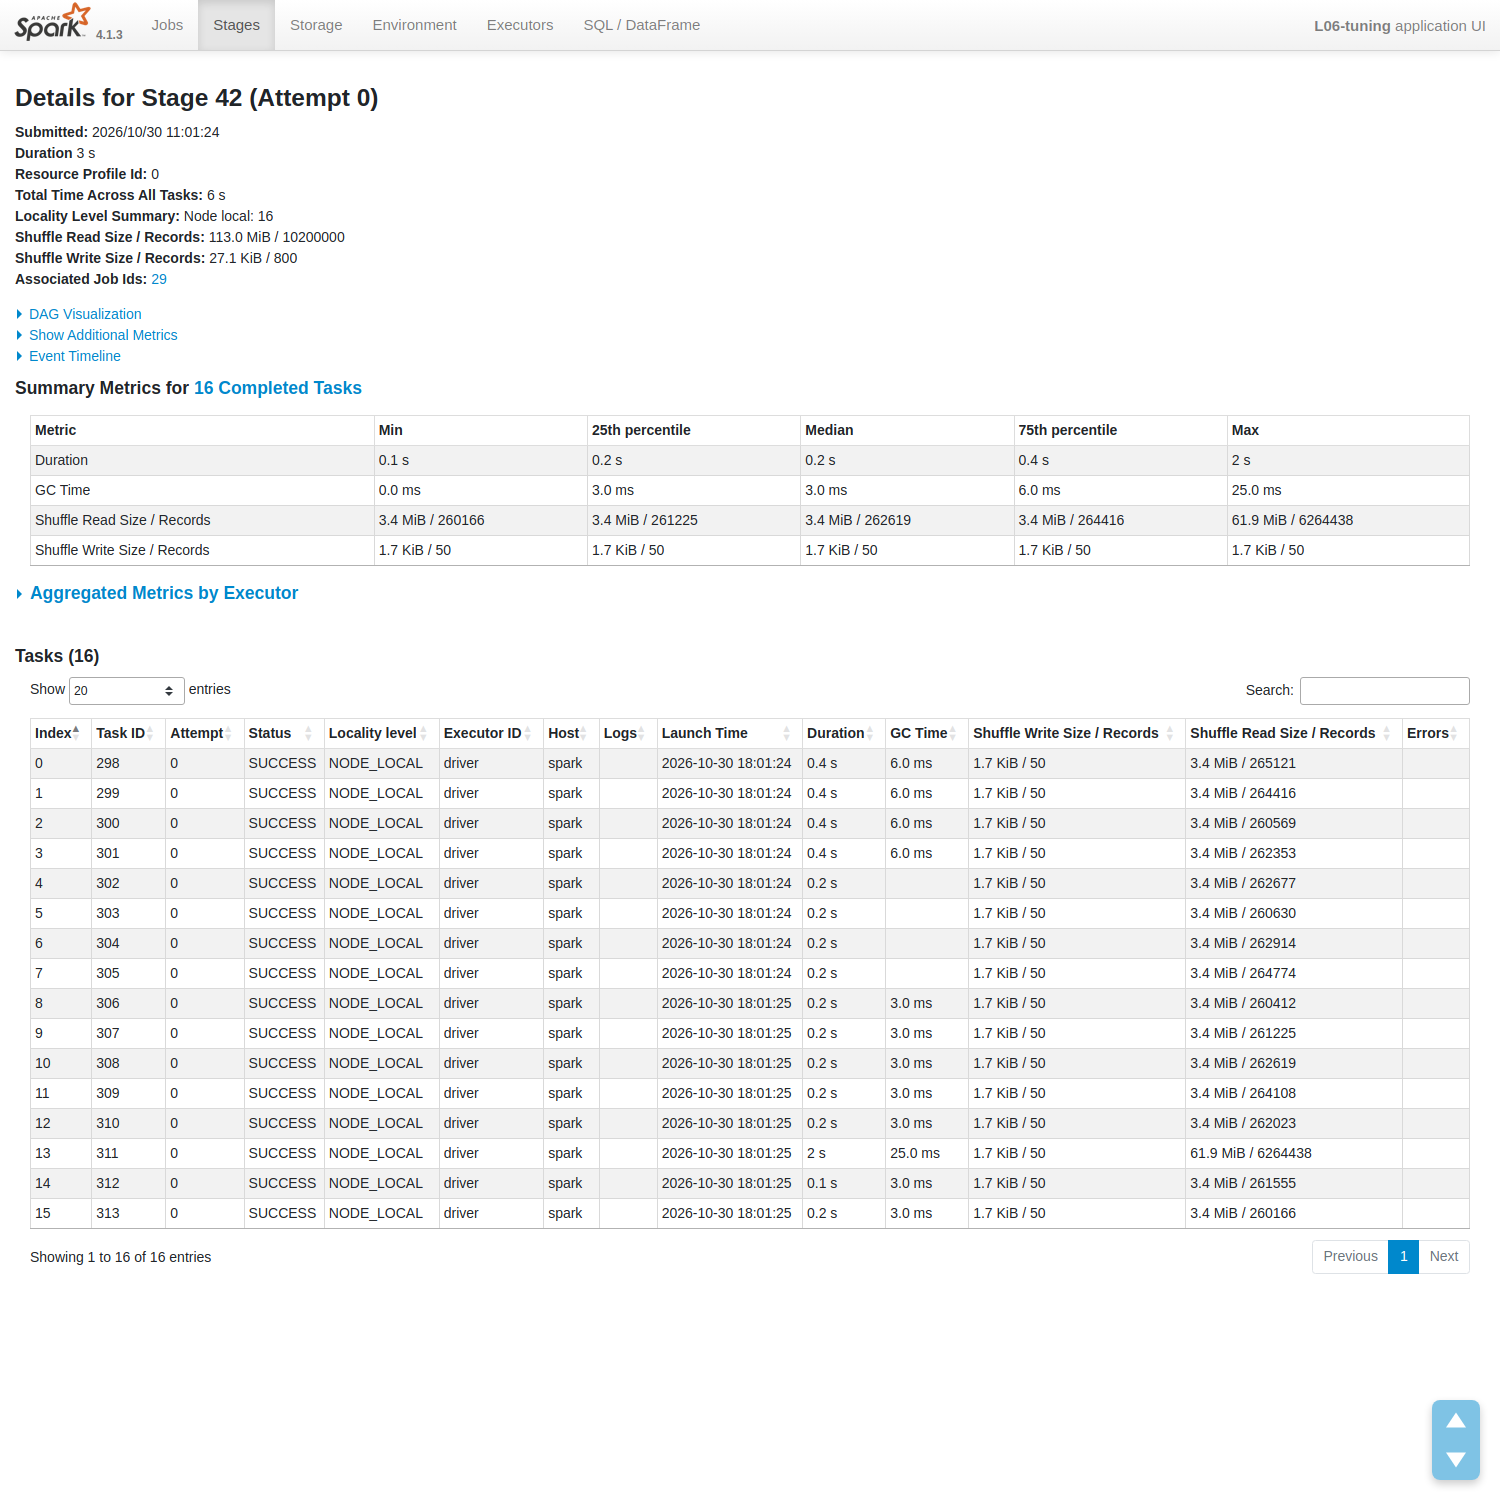
\includegraphics[width=1\linewidth,height=\textheight,keepaspectratio]{img/30_ui_e3_baseline_stage42_summary.png}
\caption{Summary Metrics của stage 42 (baseline): max 61.9 MiB /
6,264,438 bản ghi so với median 3.4 MiB / 262,619 bản ghi; task index 13
mất 2 s.}\label{fig:l06-stage42}
\end{figure}

\emph{Salting.} Rải hot key ra 64 giá trị salt làm task max giảm gần một
nửa và số bản ghi lớn nhất mỗi task chỉ còn chưa tới một triệu
(Hình~\ref{fig:l06-stage46}). Bù lại, median tăng lên 590 ms vì
partition nào cũng nhận thêm một phần hot key, lại thêm chi phí
\texttt{rand()}, cột join phụ và 64 bản sao dòng dim. Kết quả là thời
gian tổng gần như đứng yên (4.01 s so với 4.10 s). Tổng \texttt{amount}
vẫn đúng (500061629), nghĩa là salting không làm sai kết quả.

\begin{figure}
\centering
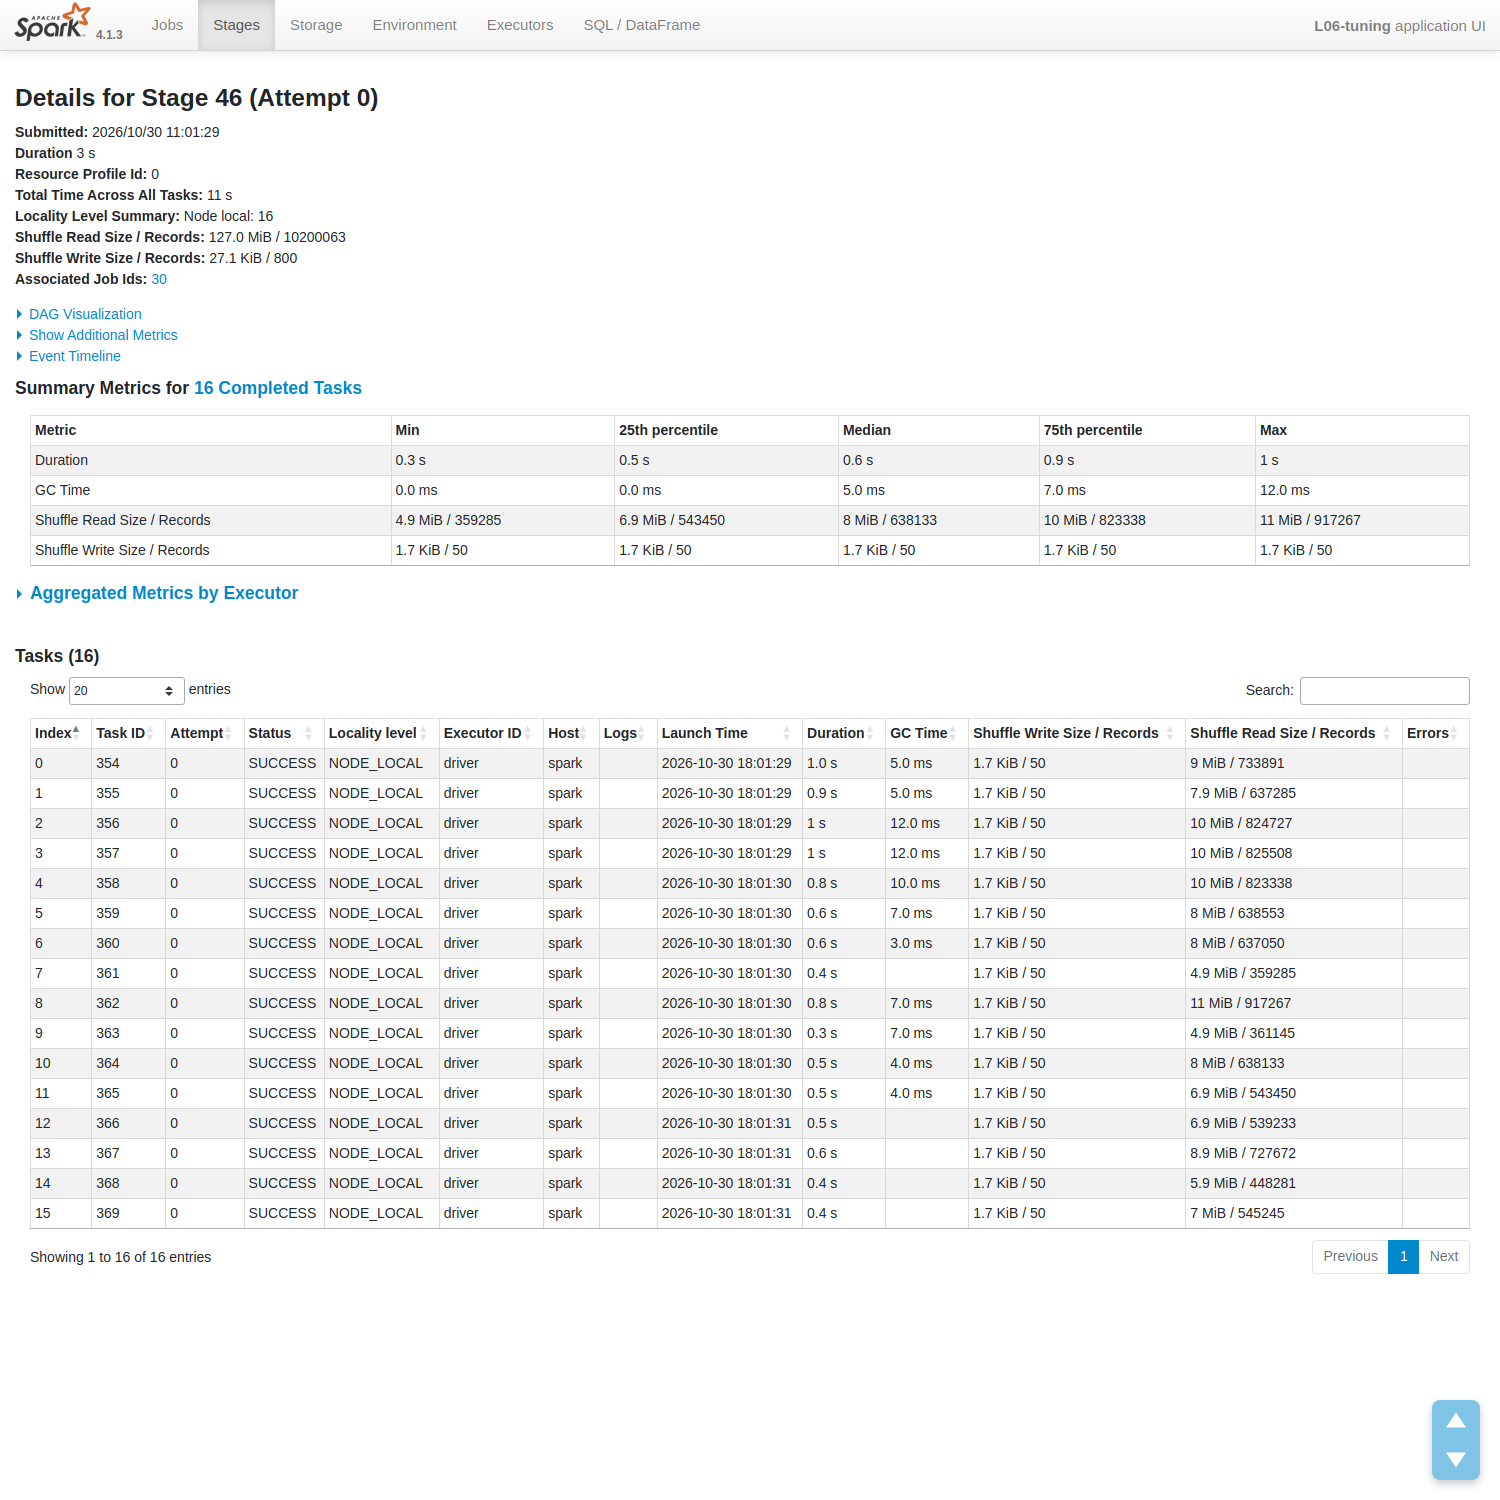
\includegraphics[width=1\linewidth,height=\textheight,keepaspectratio]{img/31_ui_e3_salted_stage46_summary.png}
\caption{Summary Metrics của stage 46 (salting 64): phân bố bản ghi đều
hơn, max 917,267 bản ghi, nhưng median thời gian task tăng lên 590
ms.}\label{fig:l06-stage46}
\end{figure}

\emph{AQE skew join.} Kế hoạch cuối có
\texttt{SortMergeJoin(skew=}\allowbreak{}\texttt{true)}\allowbreak{}, và
\texttt{AQEShuffleRead} báo \emph{number of skewed partitions: 1, skewed
partition splits: 4, number of partitions: 19}
(Hình~\ref{fig:l06-e3aqe}). Phía fact ghi 10,000,000 bản ghi shuffle
(111.2 MiB); sau khi đọc, partition có median 3.5 MiB và max 16.7 MiB. Ở
stage 52 (Hình~\ref{fig:l06-stage52}), số bản ghi lớn nhất mỗi task xấp
xỉ một phần tư của baseline, đúng với 4 split. Thời gian tổng còn
\textbf{2.22 s, nhanh gần gấp đôi baseline}, và không phải sửa dòng truy
vấn nào. Lúc đầu chúng tôi để ngưỡng mặc định thì AQE không tách gì, vì
partition nóng chỉ có 61.9 MiB, thấp hơn nhiều so với mức 256 MB mặc
định. Vì vậy phải hạ ngưỡng như đã nêu ở Mục~\ref{sec:l06-method}.

\begin{figure}
\centering
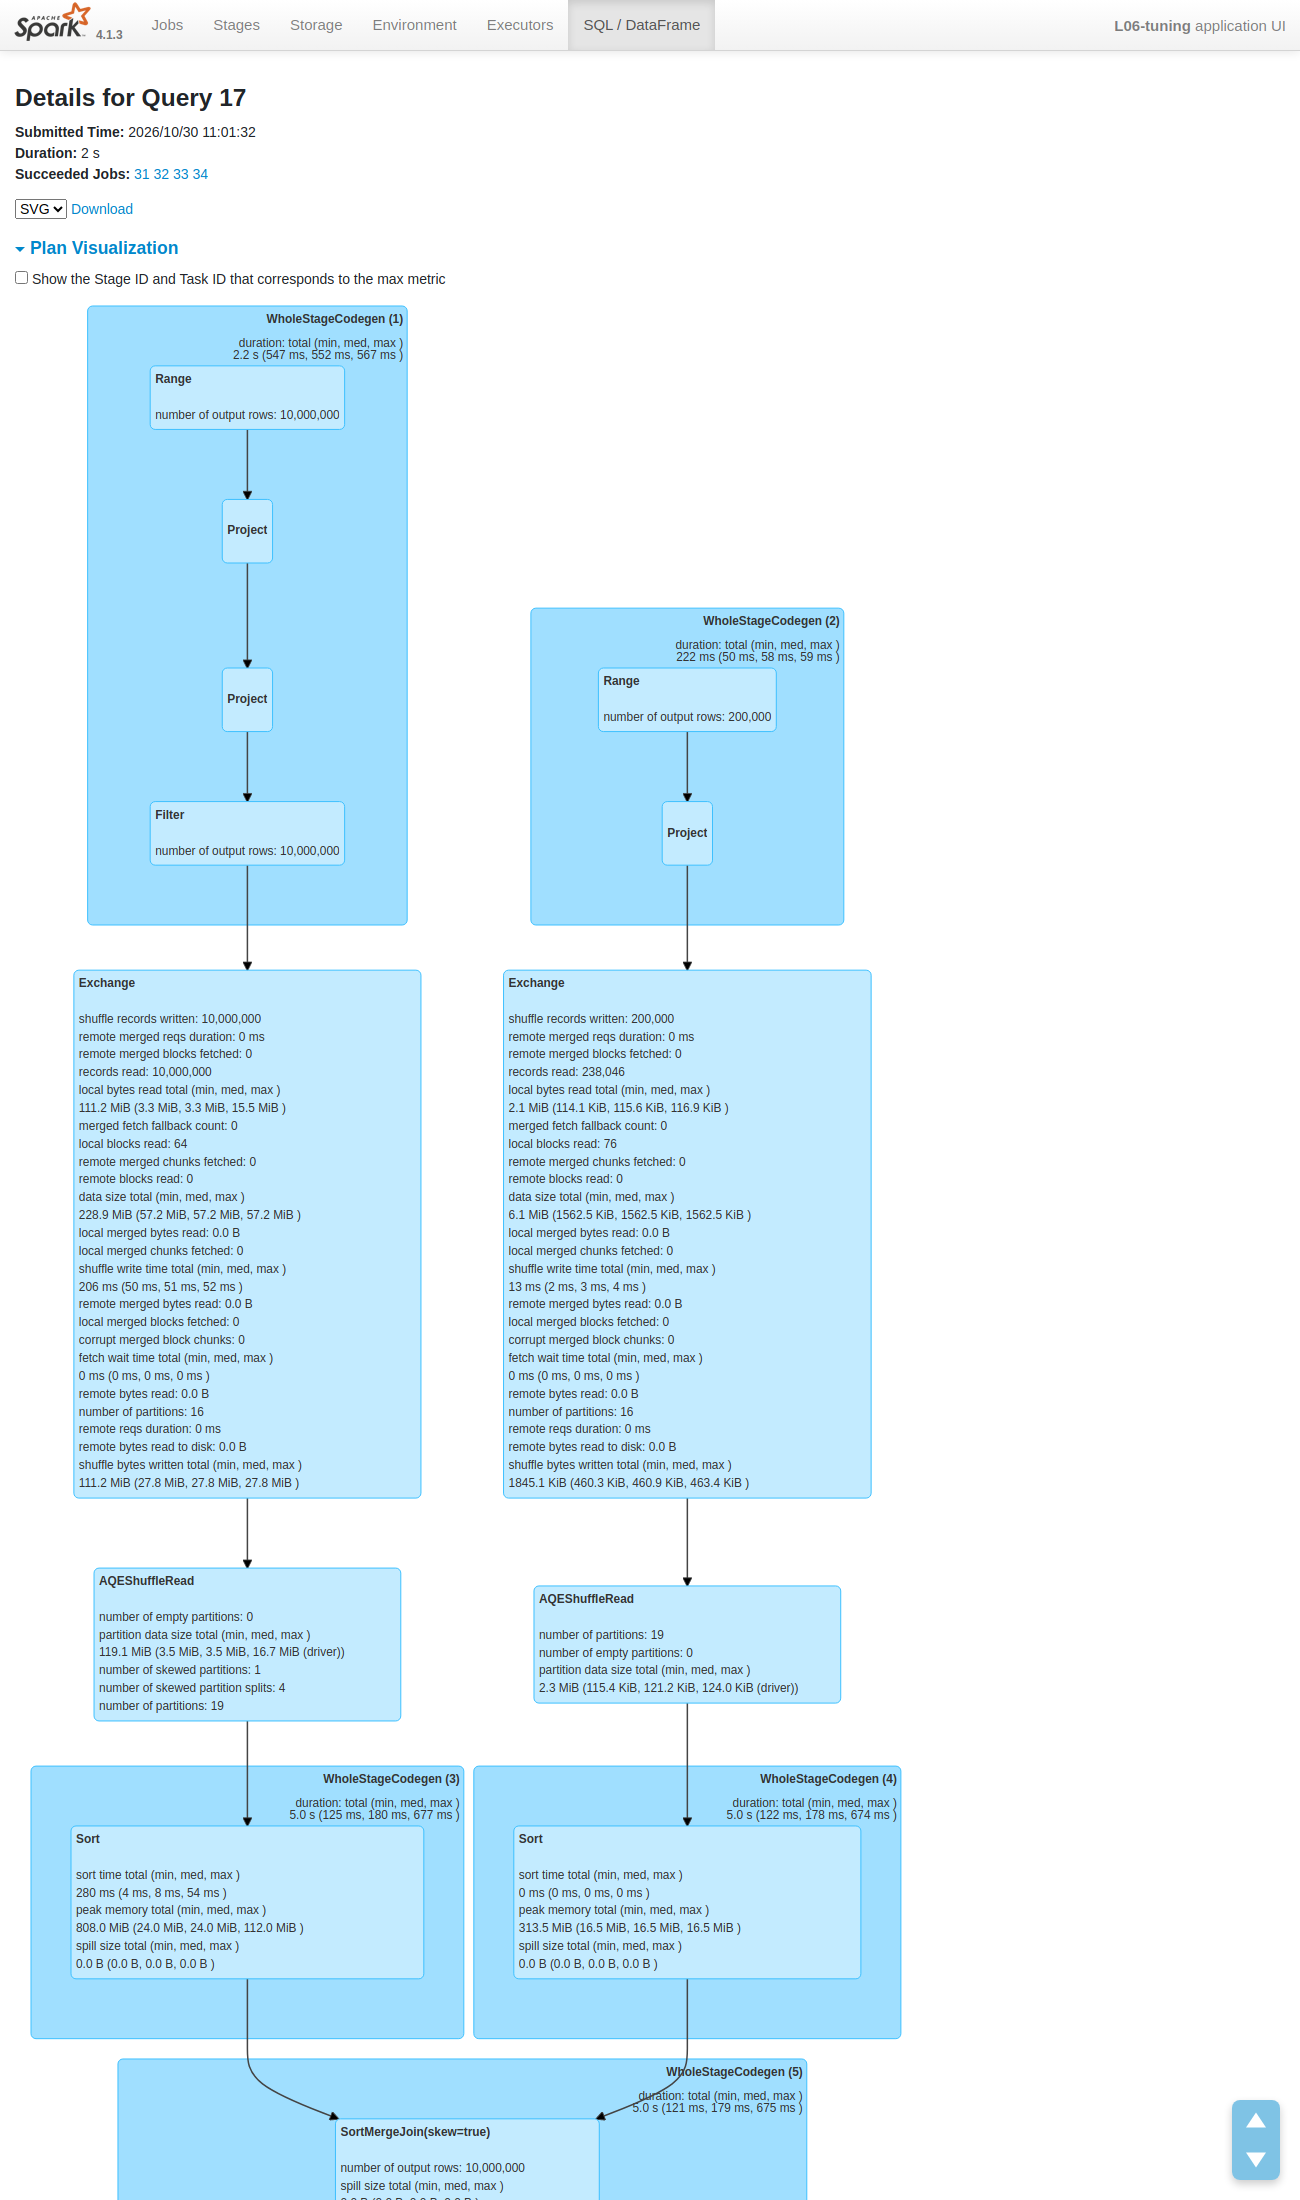
\includegraphics[width=0.85\linewidth,height=\textheight,keepaspectratio]{img/26_ui_e3_aqe_skew_join.png}
\caption{Kế hoạch E3 với AQE skew join: \texttt{AQEShuffleRead} báo 1
partition lệch được tách thành 4 split (16 thành 19 partition), sau đó
là
\texttt{SortMergeJoin(skew=}\allowbreak{}\texttt{true)}\allowbreak{}.}\label{fig:l06-e3aqe}
\end{figure}

\begin{figure}
\centering
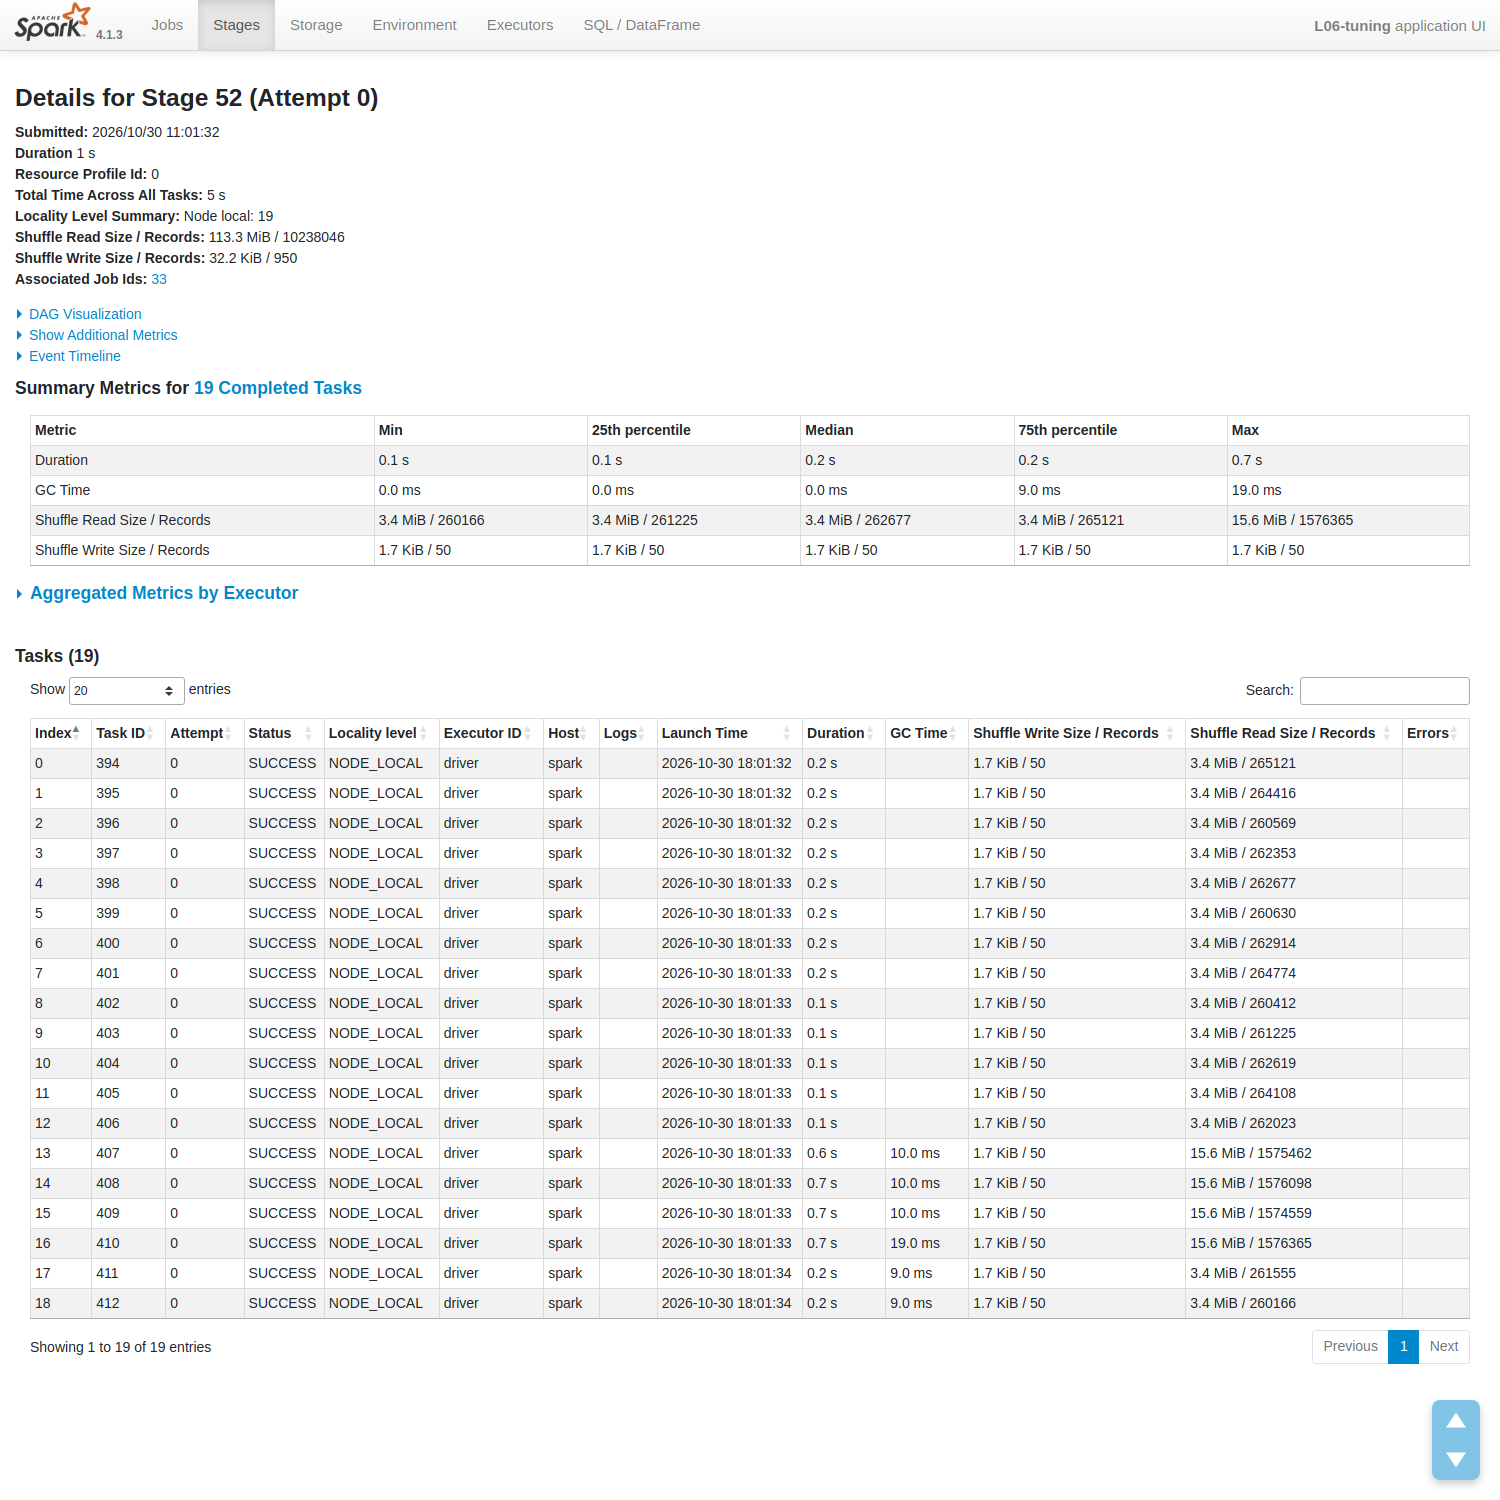
\includegraphics[width=1\linewidth,height=\textheight,keepaspectratio]{img/32_ui_e3_aqe_stage52_summary.png}
\caption{Summary Metrics của stage 52 (AQE skew join): max 682 ms và
1,576,365 bản ghi mỗi task.}\label{fig:l06-stage52}
\end{figure}

\subsection{E4: repartition và coalesce trước khi
ghi}\label{e4-repartition-vuxe0-coalesce-trux1b0ux1edbc-khi-ghi}

\texttt{repartition(64)} chậm nhất vì vừa có một shuffle đầy đủ vừa ghi
64 file nhỏ. \texttt{coalesce(4)} không shuffle nên nhanh nhất, nhưng
chỉ ra 3 file chứ không phải 4. Ban đầu chúng tôi nghĩ có lỗi; xem lại
thì file Parquet đầu vào chỉ có 3 row group nên một trong 4 partition
đầu vào rỗng. \texttt{coalesce(1)} dồn cả bước đọc lẫn bước ghi vào một
task duy nhất và mất hết song song. \texttt{repartition(4)} cho 4 file
đều nhau, đổi lại phải trả thêm một shuffle (Bảng~\ref{tbl:l06-full}).

\subsection{E5: cache}\label{e5-cache}

DataFrame ``cleaned'' gồm một phép lọc và \texttt{dropDuplicates} trên
năm cột, tức là shuffle toàn bộ khoảng 3 triệu dòng. Nó được dùng cho ba
phép tổng hợp: theo giờ, theo \texttt{PULocationID} và theo
\texttt{payment\_type}. Không cache thì dedup chạy lại ba lần. Có cache
thì \texttt{count()} để materialize mất 3.42 s và trả về 2,869,714 dòng,
sau đó ba truy vấn chỉ còn \textbf{0.99 s}. Tab Storage
(Hình~\ref{fig:l06-storage}) cho thấy 8/8 partition đã được cache (100
\%), chiếm 59.4 MiB bộ nhớ và 0.0 B đĩa, mức
\texttt{Disk\ Memory\ Serialized\ 1x\ Replicated}\allowbreak{}; REST API
báo \texttt{memoryUsed} = 62,240,847 byte. Tính cả thời gian
materialize, cache vẫn lời (khoảng 4.4 s so với 6.4 s), và càng dùng lại
nhiều lần thì càng lời.

\begin{figure}
\centering
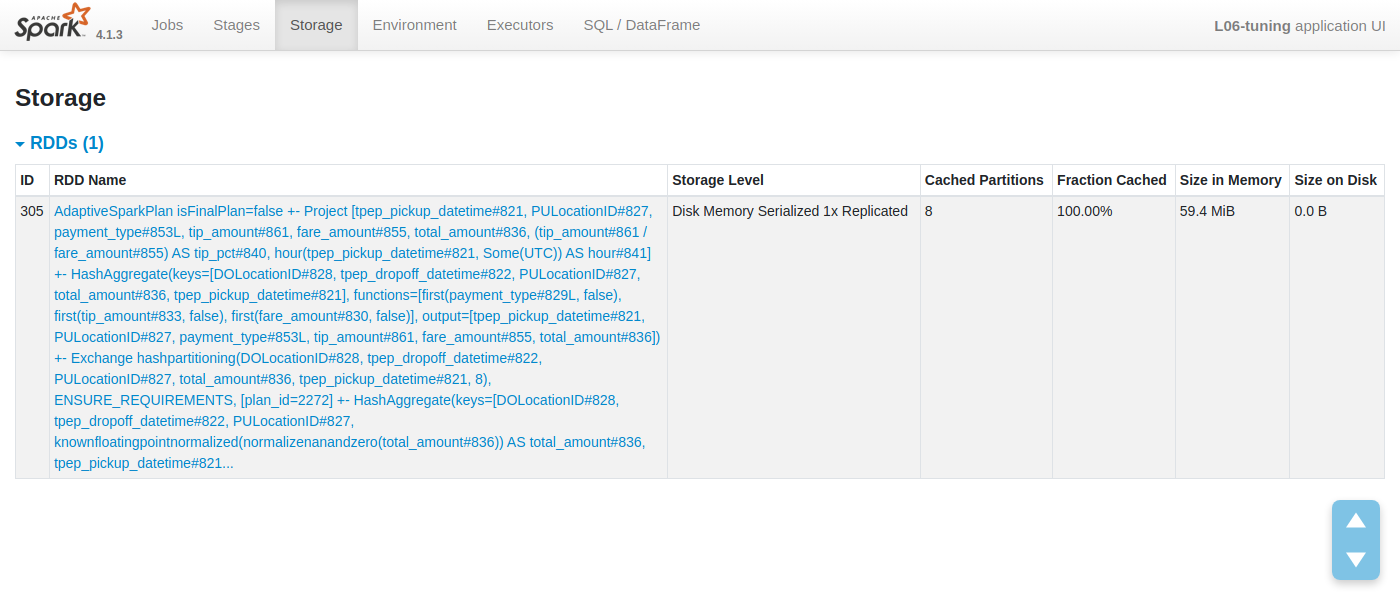
\includegraphics[width=1\linewidth,height=\textheight,keepaspectratio]{img/27_ui_storage_e5_cache.png}
\caption{Tab Storage của Spark UI: DataFrame \texttt{cleaned} được cache
8/8 partition, 100 \%, 59.4 MiB trong bộ nhớ.}\label{fig:l06-storage}
\end{figure}

\subsection{So sánh với kết quả tham
chiếu}\label{so-suxe1nh-vux1edbi-kux1ebft-quux1ea3-tham-chiux1ebfu}

Đề bài kèm một bảng tham chiếu đo trên máy Apple M-series, Docker 4 GB,
\texttt{local{[}4{]}} (Bảng~\ref{tbl:l06-ref}). Thời gian trên máy chúng
tôi cao hơn khoảng 1.3 đến 1.9 lần, có thể do khác phần cứng và có thêm
lớp WSL2. Mọi xu hướng thì khớp: trong E1, 200 partition chậm nhất và
AQE bắt kịp bản chỉnh tay; trong E2, gợi ý broadcast nhanh nhất;
baseline E3 có tỉ lệ max/median lớn, salting không rút được thời gian
tổng còn AQE skew join nhanh nhất; và \texttt{coalesce(4)} cũng ra 3
file. Chỗ khác là số task của AQE skew join (27 so với 43), vì số
partition sau khi tách phụ thuộc kích thước partition thực tế lúc chạy.

\begin{longtable}[]{@{}
  >{\raggedright\arraybackslash}p{(\linewidth - 4\tabcolsep) * \real{0.3333}}
  >{\raggedright\arraybackslash}p{(\linewidth - 4\tabcolsep) * \real{0.3333}}
  >{\raggedright\arraybackslash}p{(\linewidth - 4\tabcolsep) * \real{0.3333}}@{}}
\caption{\label{tbl:l06-ref}So sánh với bảng kết quả tham chiếu của bài
lab.}\tabularnewline
\toprule\noalign{}
\begin{minipage}[b]{\linewidth}\raggedright
Chỉ số
\end{minipage} & \begin{minipage}[b]{\linewidth}\raggedright
Tham chiếu
\end{minipage} & \begin{minipage}[b]{\linewidth}\raggedright
Lần 2
\end{minipage} \\
\midrule\noalign{}
\endfirsthead
\toprule\noalign{}
\begin{minipage}[b]{\linewidth}\raggedright
Chỉ số
\end{minipage} & \begin{minipage}[b]{\linewidth}\raggedright
Tham chiếu
\end{minipage} & \begin{minipage}[b]{\linewidth}\raggedright
Lần 2
\end{minipage} \\
\midrule\noalign{}
\endhead
\bottomrule\noalign{}
\endlastfoot
E1, 200 partition, AQE off & 1.29 s & 2.20 s \\
E1, AQE on & 0.21 s & 0.53 s \\
E2, broadcast hint & 0.24 s & 0.40 s \\
E3 baseline (median / max task) & 110 / 1,263 ms & 165 / 2,366 ms \\
E3 salting & 2.97 s & 4.01 s \\
E3 AQE skew join (thời gian, task) & 1.73 s, 43 task & 2.22 s, 27
task \\
E4 coalesce(4) & 1.85 s, 3 file & 3.12 s, 3 file \\
E5 không cache / có cache & 4.11 / 0.70 s & 6.40 / 0.99 s \\
\end{longtable}

\section{Thảo luận}\label{sec:l06-discussion}

\subsection{Vì sao 200 partition chậm, và vì sao không nên đặt 1
partition dù nó chạy nhanh?}\label{sec:l06-q1}

Kết quả \texttt{groupBy(PU,\ DO)} chỉ có khoảng 20 nghìn nhóm, dữ liệu
shuffle chưa tới 1.2 MiB. Chia nhỏ chừng đó ra 200 phần thì mỗi task
reduce chỉ làm việc khoảng 6 ms, còn chi phí lập lịch, serialize và khởi
tạo của 204 task lớn hơn phần việc thật. Vì vậy bản này chậm hơn bản 8
partition khoảng 6.7 lần (Bảng~\ref{tbl:l06-full}). Một partition chạy
nhanh ở đây chỉ vì shuffle quá nhỏ. Với dữ liệu thật, một reducer phải
ôm toàn bộ dữ liệu shuffle: không có song song, dễ spill ra đĩa và dễ
OOM. Thực tế nên nhắm khoảng 100--200 MB mỗi partition shuffle, hoặc để
AQE tự quyết.

\subsection{\texorpdfstring{\texttt{AQEShuffleRead\ coalesced}\allowbreak{}
làm gì, và AQE biết gì mà planner tĩnh không
biết?}{AQEShuffleRead coalesced làm gì, và AQE biết gì mà planner tĩnh không biết?}}\label{sec:l06-q2}

Khi stage map của shuffle chạy xong, AQE có kích thước thật của từng
partition shuffle. \texttt{AQEShuffleRead\ coalesced}\allowbreak{} cho
một reducer đọc gộp nhiều partition nhỏ liền kề cho tới khi đạt
\texttt{advisoryPartitionSizeInBytes}\allowbreak{}. Trong E1, 200
partition chỉ còn một task reduce và tổng số task giảm từ 204 xuống 5
(Hình~\ref{fig:l06-e1on}). Planner tĩnh chỉ có ước lượng dựa trên kích
thước file, và ước lượng này hay sai sau filter, join hoặc aggregate.

\subsection{Con số nào cho thấy skew, vì sao salting không rút ngắn thời
gian tổng trên 4 core, và khi nào salting thắng?}\label{sec:l06-q3}

Bằng chứng là chênh lệch giữa task max và median ở stage join:
\textbf{2,366 ms so với 165 ms}, và task chậm nhất đọc 6,264,438 bản ghi
trong khi median là 262,619 (Bảng~\ref{tbl:l06-quantiles},
Hình~\ref{fig:l06-stage42}).

Salting cắt task max xuống 1,197 ms nhưng thời gian tổng gần như không
đổi. Một phần là vì salting thêm việc ở mọi chỗ: \texttt{rand()} cho
từng dòng, thêm cột join, nhân dòng dim lên 64 lần. Phần lớn hơn là
khoảng 6 triệu dòng hot vẫn phải chia trên 16 partition chạy trên 4
core. Tổng khối lượng việc không giảm, chỉ được chia lại, nên median
tăng từ 165 lên 590 ms. Lần chạy đầu cũng vậy: salting chỉ nhanh hơn
baseline một chút (4.28 s so với 4.62 s), còn bảng tham chiếu thậm chí
ghi salting chậm hơn (2.97 s so với 2.45 s). Salting sẽ thắng rõ khi có
nhiều core và nhiều partition, vì lúc đó một straggler giữ hàng trăm
executor rảnh. Nó cũng có lợi khi mỗi dòng xử lý nặng (dòng rộng, join
many-to-many, có spill) hoặc khi skew nặng hơn, ví dụ 90 \% hot.

\subsection{AQE nhận ra partition lệch thế nào, xử lý ra sao, và kém
salting ở đâu?}\label{sec:l06-q4}

Một partition bị coi là lệch khi nó vừa lớn hơn
\texttt{skewedPartitionFactor}\allowbreak{} lần median, vừa lớn hơn
\texttt{skewedPartitionThresholdInBytes}\allowbreak{}. Mặc định là 5 lần
và 256 MB; bài lab hạ xuống 3 lần và 16 MB cho vừa dữ liệu nhỏ.
Partition hot ở đây là 61.9 MiB so với median 3.4 MiB, thỏa cả hai điều
kiện. AQE tách partition đó theo các khoảng map output (4 split, nên 16
partition thành 19), rồi nhân bản partition tương ứng ở phía còn lại; kế
hoạch hiện
\texttt{SortMergeJoin(skew=}\allowbreak{}\texttt{true)}\allowbreak{}
(Hình~\ref{fig:l06-e3aqe}). Số bản ghi lớn nhất mỗi task còn 1,576,365,
xấp xỉ 6,264,438 / 4.

AQE có mấy giới hạn mà salting không có. Nó chỉ áp dụng cho join có
shuffle ở cả hai phía (sort-merge hoặc shuffled hash join), và không
tách được phía phải giữ nguyên của outer join. Ngưỡng phải hợp với dữ
liệu, nếu không nó sẽ không kích hoạt; chúng tôi đã gặp đúng chuyện này
ở E3. Quan trọng nhất là AQE không xử lý skew trong \texttt{groupBy} hay
skew phát sinh sau join, trong khi salting hoặc aggregate hai pha làm
được.

\subsection{Khi nào không nên broadcast dù một phía
``nhỏ''?}\label{sec:l06-q5}

Không nên broadcast trong các trường hợp sau:

\begin{itemize}
\tightlist
\item
  bảng vẫn lớn khi nằm trong bộ nhớ: driver phải collect rồi gửi bản sao
  tới mọi executor, dễ OOM ở driver hoặc broadcast timeout;
\item
  thống kê đánh giá thấp kích thước thật, ví dụ sau filter hoặc UDF;
\item
  join là full outer join (không hỗ trợ), hoặc phía cần broadcast lại là
  phía được giữ của outer join;
\item
  join chạy lặp lại trên dữ liệu thay đổi, nên mỗi lần phải dựng lại
  broadcast.
\end{itemize}

Bảng zones trong E2 chỉ có 265 dòng và không rơi vào trường hợp nào ở
trên, nên broadcast là đúng (Hình~\ref{fig:l06-e2bhj}).

\subsection{\texorpdfstring{\texttt{repartition(n)} hay
\texttt{coalesce(n)}: cái nào shuffle, cái nào tạo file lệch, cái nào
làm giảm song song stage
trước?}{repartition(n) hay coalesce(n): cái nào shuffle, cái nào tạo file lệch, cái nào làm giảm song song stage trước?}}\label{sec:l06-q6}

\texttt{repartition(n)} luôn shuffle. Nhờ vậy partition cân bằng (4 file
đều nhau) và stage trước vẫn giữ mức song song, cái giá là thêm một
shuffle. \texttt{coalesce(n)} gộp partition có sẵn mà không shuffle nên
rẻ hơn, nhưng file ra có thể lệch: ở E4 chỉ có 3 file vì đầu vào chỉ có
3 row group. Vì \texttt{coalesce} là narrow dependency, nó kéo luôn
stage trước về cùng số task. \texttt{coalesce(1)} đọc và ghi trong một
task duy nhất, mất 6,800 ms (Bảng~\ref{tbl:l06-full}).

\subsection{Vì sao cache có ích trong E5, còn cache một DataFrame rẻ thì
thường không?}\label{sec:l06-q7}

DataFrame được cache trong E5 là kết quả của một bước đắt
(\texttt{dropDuplicates}, shuffle toàn bộ khoảng 3 triệu dòng) và được
dùng lại ba lần. Cache nên bước này chỉ chạy một lần thay vì ba
(Hình~\ref{fig:l06-storage}). Một phép quét Parquet chỉ lấy vài cột thì
vốn đã rẻ nhờ đọc vectorized, column pruning và predicate pushdown;
cache nó chỉ tốn thêm bộ nhớ và thời gian materialize. Nguyên tắc là
cache cái gì vừa đắt vừa được dùng lại, xong thì gọi
\texttt{unpersist()}.

\subsection{Nên tinh chỉnh gì trước khi thêm phần
cứng?}\label{sec:l06-q8}

\begin{enumerate}
\def\labelenumi{\arabic{enumi}.}
\tightlist
\item
  Đọc kế hoạch và Spark UI: tìm stage chậm nhất, spill, thời gian GC, và
  tỉ lệ task max/median để phát hiện skew (như
  Bảng~\ref{tbl:l06-quantiles}).
\item
  Lọc và chọn cột càng sớm càng tốt: partition pruning, predicate/column
  pushdown, dùng định dạng cột (Parquet/ORC).
\item
  Để partition shuffle có kích thước hợp lý: bật AQE (coalesce và skew
  join), nhắm khoảng 100--200 MB mỗi partition.
\item
  Chọn đúng kiểu join: broadcast bảng nhỏ; nếu có skew thì dùng AQE skew
  join, salting, hoặc tách hot key.
\item
  Tránh UDF Python (dùng hàm built-in hoặc pandas UDF), chỉ cache khi
  cần, và tránh sinh file nhỏ khi ghi (repartition hoặc compaction).
\end{enumerate}

\subsection{Hạn chế của thực nghiệm}\label{sec:l06-limits}

Mọi thứ chạy local trên một máy 4 core, không có chi phí mạng, nên chênh
lệch giữa các chiến lược nhỏ hơn nhiều so với trên cluster. Vì thế cột
max/median đáng tin hơn thời gian tuyệt đối. Dữ liệu nhỏ (một tháng
taxi, 10 triệu dòng tổng hợp) buộc phải hạ ngưỡng skew của AQE. Chỉ có
hai lần chạy, và các biến thể dưới 1 s dao động khá mạnh
(Bảng~\ref{tbl:l06-runs}). Lớp Docker/WSL2 cũng làm I/O chậm hơn so với
máy tham chiếu. Các phần mở rộng (25 triệu dòng,
\texttt{HOT\_SHARE\ =\ 0.9}, bucketing, shuffled hash join) chưa được
làm.

\section{Kết luận}\label{sec:l06-conclusion}

Ngay trên một máy, các tham số tinh chỉnh đã cho khác biệt đo được. Số
partition shuffle không hợp làm truy vấn chậm khoảng 6.7 lần, và AQE tự
sửa được việc này. Skew lộ ra rõ qua tỉ lệ task max/median khoảng 14
lần. AQE skew join giảm gần một nửa thời gian tổng mà không phải sửa mã,
còn salting chỉ chia lại việc khi số core có hạn. \texttt{coalesce} rẻ
nhưng có thể sinh file lệch và kéo stage trước về một task. Cache chỉ có
lợi khi kết quả đắt và được dùng lại.

Với một job production trên cluster 20 node, chúng tôi đề xuất:

\begin{enumerate}
\def\labelenumi{\arabic{enumi}.}
\tightlist
\item
  Luôn bật AQE (mặc định từ Spark 3.2 và trong Spark 4). Đặt
  \texttt{shuffle.}\allowbreak{}\texttt{partitions}\allowbreak{} ban đầu
  cao, khoảng 2--3 lần tổng số core (400--800), và để
  \texttt{coalescePartitions}\allowbreak{} gộp về khoảng 64--128 MB mỗi
  partition (\texttt{advisoryPartitionSizeInBytes}\allowbreak{}). Không
  đặt cứng 1 hay 8.
\item
  Broadcast các bảng dimension nhỏ. Có thể nâng
  \texttt{autoBroadcastJoinThreshold}\allowbreak{} lên khoảng 50--100 MB
  nếu executor đủ bộ nhớ, và dùng \texttt{broadcast()} khi thống kê sai.
  Không broadcast bảng vài trăm MB vì driver phải collect trước, dễ OOM.
\item
  Với skew, để AQE skew join chạy với ngưỡng mặc định (5 lần, 256 MB).
  Với hot key đã biết, hoặc skew trong \texttt{groupBy}/outer join mà
  AQE không xử lý được, dùng salting hoặc tách hot key ra xử lý riêng.
  Theo dõi tỉ lệ task max/median trong UI.
\item
  Khi ghi output, dùng \texttt{repartition(n)} hoặc
  \texttt{repartition(col)}\allowbreak{} để mỗi file khoảng 128 MB--1
  GB, tránh sinh hàng nghìn file nhỏ. Tránh \texttt{coalesce(1)} trên dữ
  liệu lớn.
\item
  Chỉ
  \texttt{persist(MEMORY\_}\allowbreak{}\texttt{AND\_}\allowbreak{}\texttt{DISK)}\allowbreak{}
  những kết quả đắt và được dùng lại ít nhất hai lần, rồi
  \texttt{unpersist()} ngay. Không cache phép quét Parquet rẻ.
\end{enumerate}

Nếu có thêm thời gian, chúng tôi muốn chạy lại E3 với 25 triệu dòng và
90 \% hot để xem ba chiến lược thay đổi thế nào khi dữ liệu lớn lên, thử
shuffled hash join với dimension lớn, dùng bucketing để bỏ
\texttt{Exchange}, và lặp lại toàn bộ trên một cluster nhiều node thật.

\section*{Tài liệu tham khảo}\label{tuxe0i-liux1ec7u-tham-khux1ea3o}
\addcontentsline{toc}{section}{Tài liệu tham khảo}

{[}1{]} M. Zaharia \emph{et al.}, ``Resilient Distributed Datasets: A
Fault-Tolerant Abstraction for In-Memory Cluster Computing,'' in
\emph{Proc. 9th USENIX Symposium on Networked Systems Design and
Implementation (NSDI)}, 2012.

{[}2{]} M. Armbrust \emph{et al.}, ``Spark SQL: Relational Data
Processing in Spark,'' in \emph{Proc. ACM SIGMOD International
Conference on Management of Data}, 2015.

{[}3{]} The Apache Software Foundation, ``Performance Tuning -- Spark
SQL, DataFrames and Datasets,'' Apache Spark Documentation.
https://spark.apache.org/docs/latest/sql-performance-tuning.html

{[}4{]} B. Chambers and M. Zaharia, \emph{Spark: The Definitive Guide}.
Sebastopol, CA: O'Reilly Media, 2018.

{[}5{]} M. Kleppmann, \emph{Designing Data-Intensive Applications}.
Sebastopol, CA: O'Reilly Media, 2017.

{[}6{]} The Apache Software Foundation, ``Monitoring and Instrumentation
(REST API),'' Apache Spark Documentation.
https://spark.apache.org/docs/latest/monitoring.html

{[}7{]} J. Dean and S. Ghemawat, ``MapReduce: Simplified Data Processing
on Large Clusters,'' in \emph{Proc. 6th Symposium on Operating Systems
Design and Implementation (OSDI)}, 2004.

\section*{Phụ lục A: Danh mục tệp nộp
kèm}\label{phux1ee5-lux1ee5c-a-danh-mux1ee5c-tux1ec7p-nux1ed9p-kuxe8m}
\addcontentsline{toc}{section}{Phụ lục A: Danh mục tệp nộp kèm}

Các tệp nộp kèm báo cáo được liệt kê ở Bảng~\ref{tbl:l06-files}.

\begin{longtable}[]{@{}
  >{\raggedright\arraybackslash}p{(\linewidth - 2\tabcolsep) * \real{0.5000}}
  >{\raggedright\arraybackslash}p{(\linewidth - 2\tabcolsep) * \real{0.5000}}@{}}
\caption{\label{tbl:l06-files}Danh mục tệp nộp kèm.}\tabularnewline
\toprule\noalign{}
\begin{minipage}[b]{\linewidth}\raggedright
Tệp
\end{minipage} & \begin{minipage}[b]{\linewidth}\raggedright
Nội dung
\end{minipage} \\
\midrule\noalign{}
\endfirsthead
\toprule\noalign{}
\begin{minipage}[b]{\linewidth}\raggedright
Tệp
\end{minipage} & \begin{minipage}[b]{\linewidth}\raggedright
Nội dung
\end{minipage} \\
\midrule\noalign{}
\endhead
\bottomrule\noalign{}
\endlastfoot
\texttt{l06\_}\allowbreak{}\texttt{experiments.}\allowbreak{}\texttt{py}\allowbreak{}
& Script thí nghiệm: E1 bật AQE, E2 gợi ý \texttt{broadcast()}, E3
salting và AQE skew join \\
\texttt{results.csv} & 34 dòng (2 lần chạy × 17 biến thể) \\
\texttt{RESULTS.md} & Bảng lần chạy thứ hai, nhận xét E1--E5, khuyến
nghị cho cluster 20 node \\
\texttt{01\_run1.txt}, \texttt{02\_run2.txt} & Log console của hai lần
chạy \\
\texttt{03\_}\allowbreak{}\texttt{e3\_}\allowbreak{}\texttt{task\_}\allowbreak{}\texttt{quantiles.}\allowbreak{}\texttt{txt}\allowbreak{}
& Phân vị thời gian task và số bản ghi shuffle mỗi task của ba stage
join E3 (REST API) \\
\texttt{img/} & Ảnh chụp console và Spark UI \\
\end{longtable}

\section*{Phụ lục B: Trích đoạn mã
nguồn}\label{phux1ee5-lux1ee5c-b-truxedch-ux111oux1ea1n-muxe3-nguux1ed3n}
\addcontentsline{toc}{section}{Phụ lục B: Trích đoạn mã nguồn}

Trong
\texttt{l06\_}\allowbreak{}\texttt{experiments.}\allowbreak{}\texttt{py}\allowbreak{},
ở E1 chúng tôi bật lại AQE nhưng giữ 200 partition để xem AQE tự gộp:

\begin{Shaded}
\begin{Highlighting}[]
\NormalTok{set\_conf(spark\_\_sql\_\_adaptive\_\_enabled}\OperatorTok{=}\VariableTok{True}\NormalTok{, spark\_\_sql\_\_shuffle\_\_partitions}\OperatorTok{=}\DecValTok{200}\NormalTok{)}
\NormalTok{run(}\StringTok{"E1"}\NormalTok{, }\StringTok{"AQE on,  shuffle.partitions=200"}\NormalTok{, q(), }\StringTok{"AQE coalesces small shuffle partitions"}\NormalTok{)}
\end{Highlighting}
\end{Shaded}

Ở E2, ngưỡng được để ở -1 nhưng gắn gợi ý broadcast cho bảng zones:

\begin{Shaded}
\begin{Highlighting}[]
\NormalTok{set\_conf(spark\_\_sql\_\_adaptive\_\_enabled}\OperatorTok{=}\VariableTok{True}\NormalTok{, spark\_\_sql\_\_autoBroadcastJoinThreshold}\OperatorTok{={-}}\DecValTok{1}\NormalTok{)}
\NormalTok{run(}\StringTok{"E2"}\NormalTok{, }\StringTok{"AQE on,  threshold {-}1 + broadcast() hint"}\NormalTok{,}
\NormalTok{    trips\_df().join(F.broadcast(zones\_df()), F.col(}\StringTok{"PULocationID"}\NormalTok{) }\OperatorTok{==}\NormalTok{ F.col(}\StringTok{"LocationID"}\NormalTok{))}
\NormalTok{    .groupBy(}\StringTok{"Borough"}\NormalTok{).agg(F.count(}\StringTok{"*"}\NormalTok{).alias(}\StringTok{"trips"}\NormalTok{)),}
    \StringTok{"an explicit hint beats the threshold"}\NormalTok{)}
\end{Highlighting}
\end{Shaded}

Salting ở E3 chỉ gắn salt cho hot key; phía dim nhân dòng hot lên
\texttt{SALT} = 64 bản:

\begin{Shaded}
\begin{Highlighting}[]
\NormalTok{hot }\OperatorTok{=}\NormalTok{ F.col(}\StringTok{"key"}\NormalTok{) }\OperatorTok{==} \DecValTok{0}
\NormalTok{fact\_s }\OperatorTok{=}\NormalTok{ fact.withColumn(}
    \StringTok{"salt"}\NormalTok{, F.when(hot, (F.rand(seed}\OperatorTok{=}\DecValTok{5}\NormalTok{) }\OperatorTok{*}\NormalTok{ SALT).cast(}\StringTok{"int"}\NormalTok{)).otherwise(F.lit(}\DecValTok{0}\NormalTok{)))}
\NormalTok{salts }\OperatorTok{=}\NormalTok{ spark.}\BuiltInTok{range}\NormalTok{(SALT).select(F.col(}\StringTok{"id"}\NormalTok{).cast(}\StringTok{"int"}\NormalTok{).alias(}\StringTok{"salt"}\NormalTok{))}
\NormalTok{dim\_s }\OperatorTok{=}\NormalTok{ (dim.}\BuiltInTok{filter}\NormalTok{(}\OperatorTok{\textasciitilde{}}\NormalTok{hot).withColumn(}\StringTok{"salt"}\NormalTok{, F.lit(}\DecValTok{0}\NormalTok{))}
\NormalTok{         .unionByName(dim.}\BuiltInTok{filter}\NormalTok{(hot).crossJoin(salts)))}
\NormalTok{salted }\OperatorTok{=}\NormalTok{ (fact\_s.join(dim\_s, [}\StringTok{"key"}\NormalTok{, }\StringTok{"salt"}\NormalTok{])}
\NormalTok{          .groupBy(}\StringTok{"segment"}\NormalTok{).agg(F.}\BuiltInTok{sum}\NormalTok{(}\StringTok{"amount"}\NormalTok{).alias(}\StringTok{"amount"}\NormalTok{)))}
\NormalTok{run(}\StringTok{"E3"}\NormalTok{, }\SpecialStringTok{f"salted SMJ (salt=}\SpecialCharTok{\{}\NormalTok{SALT}\SpecialCharTok{\}}\SpecialStringTok{), AQE off"}\NormalTok{, salted)}
\end{Highlighting}
\end{Shaded}

Biến thể cuối của E3 bật AQE skew join và hạ ngưỡng cho vừa dữ liệu cỡ
lab, đồng thời tắt coalesce để thấy rõ phần tách:

\begin{Shaded}
\begin{Highlighting}[]
\NormalTok{set\_conf(spark\_\_sql\_\_adaptive\_\_enabled}\OperatorTok{=}\VariableTok{True}\NormalTok{,}
\NormalTok{         spark\_\_sql\_\_adaptive\_\_skewJoin\_\_enabled}\OperatorTok{=}\VariableTok{True}\NormalTok{,}
\NormalTok{         spark\_\_sql\_\_adaptive\_\_coalescePartitions\_\_enabled}\OperatorTok{=}\VariableTok{False}\NormalTok{,}
\NormalTok{         spark\_\_sql\_\_adaptive\_\_advisoryPartitionSizeInBytes}\OperatorTok{=}\StringTok{"4m"}\NormalTok{,}
\NormalTok{         spark\_\_sql\_\_adaptive\_\_skewJoin\_\_skewedPartitionThresholdInBytes}\OperatorTok{=}\StringTok{"16m"}\NormalTok{,}
\NormalTok{         spark\_\_sql\_\_adaptive\_\_skewJoin\_\_skewedPartitionFactor}\OperatorTok{=}\DecValTok{3}\NormalTok{)}
\NormalTok{run(}\StringTok{"E3"}\NormalTok{, }\StringTok{"skewed SMJ, AQE skewJoin on"}\NormalTok{,}
\NormalTok{    fact.join(dim, }\StringTok{"key"}\NormalTok{).groupBy(}\StringTok{"segment"}\NormalTok{).agg(F.}\BuiltInTok{sum}\NormalTok{(}\StringTok{"amount"}\NormalTok{)),}
    \StringTok{"look for AQEShuffleRead (skewed) in the SQL tab"}\NormalTok{)}
\end{Highlighting}
\end{Shaded}


\end{document}
